\chapter{Анализ результатов расчётов}\label{ch:ResultsAnalysis} 

\section{Стратегия исследования и обезразмеривание}\label{sec:ResultsAnalysis/Strategy}

В дальнейших расчётах, для изучения качественных различий между классической (локальной) и нелокальной моделями, проведём процедуру обезразмеривания основных расчётых параметров уравнений теплопроводности (\ref{eq:StationaryHeatEquation}) и равновесия (\ref{eq:EquilibriumEquation}), где безразмерные параметры будем обозначать теми же символами, но с чертой над ними
\begin{gather*}
	\overline{\boldsymbol{x}} = \dfrac{\boldsymbol{x}}{L},
	\quad
	\overline{T} = \dfrac{T}{T_0},
	\quad
	\overline{\boldsymbol{\lambda}} = \dfrac{\widehat{\boldsymbol{\lambda}}}{\lambda_0},
	\quad
	\overline{E} = \dfrac{E}{\sigma_0},
	\quad
	\overline{\alpha}^T = \alpha^T T_0.
\end{gather*}
Здесь $L$ --- характерный размер области; $T_0$ --- нормализующий множитель для температуры; $\lambda_0$ --- нормализующий множитель для тензора теплопроводности; $\sigma_0$~---~нормализующий множитель для напряжений. Также чертой сверху будем обозначать безразмерные величины, которые образуются посредством комбинации приведённых выше безразмерных параметров. В расчётах, если не оговорено иначе, примем безразмерный тензор теплопроводности $\overline{\boldsymbol{\lambda}} = \widehat{\textbf{I}}_2$, безразмерный модуль Юнга $\overline{E} = 400$, коэффициент Пуассона $\nu = 0.3$ и безразмерный температурный коэффициент линейного расширения $\overline{\alpha}^T = 2.5 \cdot 10^{-3}$.

Стратегия исследования модели подразумевает вариацию основных параметров при фиксации всех остальных. Весовой параметр $p_1$ и радиус нелокальности $\overline{r}$ будем варьировать линейно, причём для параметра $p_1$ будут рассмотрены четыре сценария: отсутствие нелокальных эффектов ($p_1 = 1$); локальное слагаемое преобладает над нелокальным ($p_1 = 0.75$); локальное и нелокальное слагаемые имеют одинаковый вес ($p_1 = 0.5$); и нелокальное слагаемое преобладает над локальным ($p_1 = 0.25$). Полностью нелокальную постановку ($p_1 = 0$) рассматривать не будем, так как это приводит к некорректно поставленным краевым задачам, что требует дополнительных рассуждений при их решении.

Все дальнейшие расчёты будем проводить с использованием квадратичных серендиповых элементов, где характерный размер элемента будет указан отдельно для каждой решаемой задачи. Также, по возможности, для наглядности все расчётные параметры модели будут указаны прямо на рисунках с решениями. С целью уменьшения дублирования полученных выводов, некоторые промежуточные результаты будут учтены при решении последующих задач.

\section{Основные особенности решений}\label{sec:ResultsAnalysis/KeyFeatures}

Рассмотрим изучение нелокальных моделей теплопроводности и упругости с решения серии задач на единичном квадрате $S = \left\{ \overline{\boldsymbol{x}} \ | \ -0.5 \leqslant \overline{x}_1, \overline{x}_2 \leqslant 0.5 \right\}$. Решения будем искать на равномерной сетке $S_h$ с характерным размером элементов $h = 0.004$. Поставим граничные и интегральное условия для уравнения теплопроводности
\begin{gather*}
	\boldsymbol{n} \cdot \overline{\boldsymbol{q}} |_{\overline{x}_1 = -0.5} = 1,
	\quad
	\boldsymbol{n} \cdot \overline{\boldsymbol{q}} |_{\overline{x}_1 = 0.5} = -1,
	\quad
	\int\limits_S T dS = 0,
\end{gather*}
а также сформулируем граничные и геометрические условия для уравнения равновесия
\begin{gather*}
	n_j \overline{\sigma}_{j1} |_{\overline{x}_1 = -0.5} = -1,
	\quad
	n_j \overline{\sigma}_{j1} |_{\overline{x}_1 = 0.5} = 1,
	\quad
	\overline{u}_1 |_{\overline{x}_1 = 0} = 0,
	\quad
	\overline{u}_2 |_{\overline{x}_2 = 0} = 0.
\end{gather*}

Для определения относительного отклонения будем рассматривать нормированную разность нелокального и локального решений в сечениях вдоль оси нагружения, где в качестве нормировочного множителя будет выступать максимальное по модулю значение локального решения
\begin{gather*}
	\widetilde{T} = \dfrac{\overline{T}^{NL} - \overline{T}^L}{\max\limits_{\boldsymbol{x} \in S} \left| \overline{T}^L \right|},
	\quad
	\widetilde{u}_1 = \dfrac{\overline{u}^{NL}_1 - \overline{u}^L_1}{\max\limits_{\boldsymbol{x} \in S} \left| \overline{u}^L_1 \right|}.
\end{gather*}
Сравнительный анализ для уравнения теплопроводности и равновесия будем проводить одновременно, так как наблюдаемые в решениях явления весьма похожи.

Начнём изучение решений с вариации весового параметра модели $p_1$. Как показано на Рис.~\ref{fig:VariationP1}, увеличение вклада нелокального влияния увеличивает отклонение решений относительно классического. Причём при параметре $p_1 = 0.25$ наблюдаем осциляции решения вблизи границ области, где также наблюдаем кромочный эффект, характеризующийся резкими изменениями решения.

\begin{figure}[ht]
    \begin{minipage}[b][][b]{0.49\linewidth}\centering
        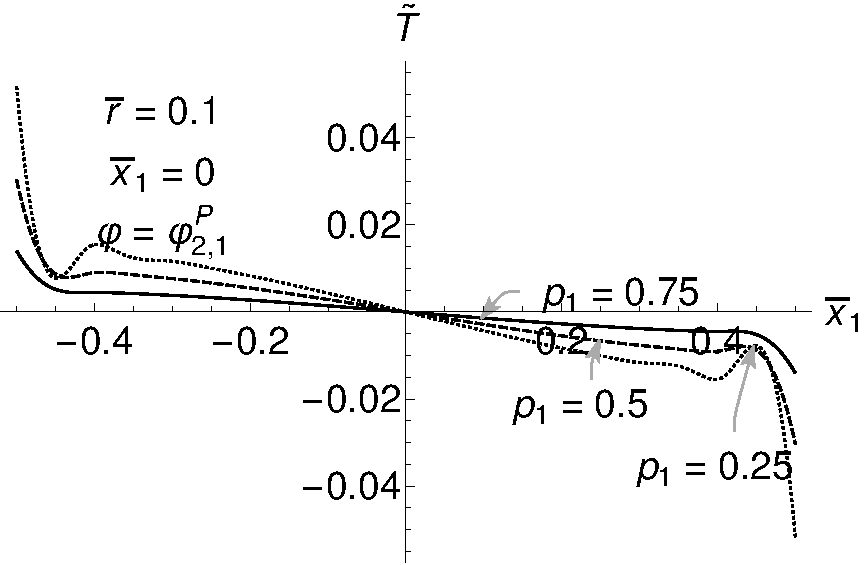
\includegraphics[width=\linewidth]{pics/TVarP1.pdf} \\ а)
    \end{minipage}
    \hfill
    \begin{minipage}[b][][b]{0.49\linewidth}\centering
        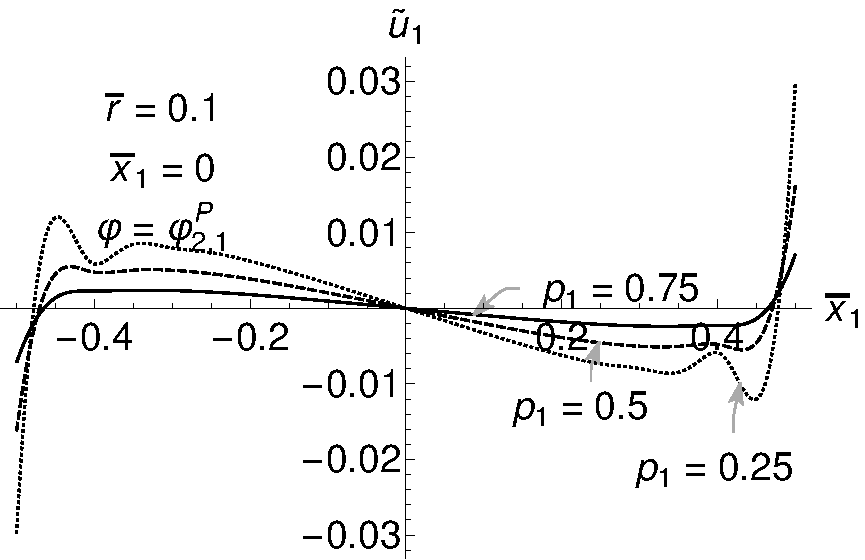
\includegraphics[width=\linewidth]{pics/U1VarP1.pdf} \\ б)
    \end{minipage}
    \caption{Решения при вариации весового параметра параметра $p_1$}
    \label{fig:VariationP1}
\end{figure}

Вариация радиуса нелокальности, представленная на Рис.~\ref{fig:VariationR}, также увеличивает отклонения, но вместе с тем и ширину кромочного эффекта пропорционально радиусу.

\begin{figure}[ht]
    \begin{minipage}[b][][b]{0.49\linewidth}\centering
        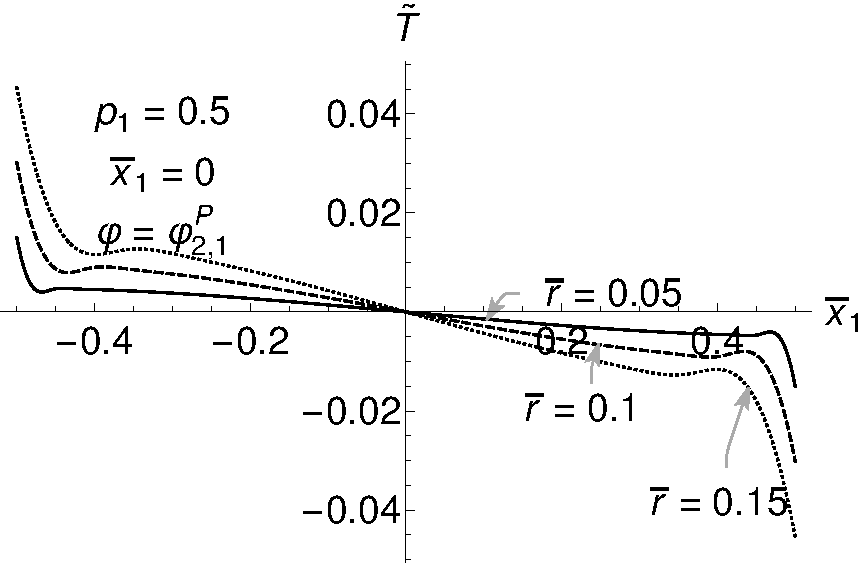
\includegraphics[width=\linewidth]{pics/TVarR.pdf} \\ а)
    \end{minipage}
    \hfill
    \begin{minipage}[b][][b]{0.49\linewidth}\centering
        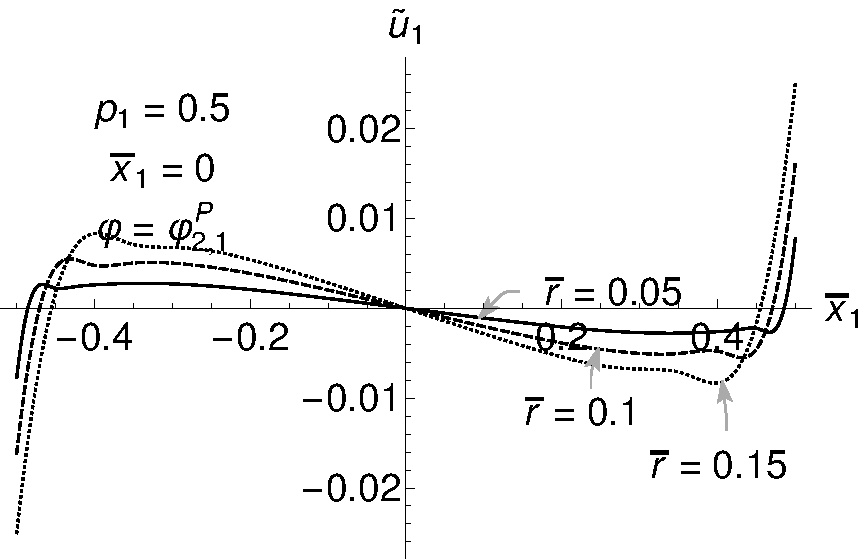
\includegraphics[width=\linewidth]{pics/U1VarR.pdf} \\ б)
    \end{minipage}
    \caption{Решения при вариации радиуса нелокальности $\overline{r}$}
    \label{fig:VariationR}
\end{figure}

Заметим, что в двумерном случае, отклонения также зависят и от рассматриваемого сечения. На Рис.~\ref{fig:VariationX2} представлены распределения температуры и перемещения в различных сечения и при приближении к свободным от условий границам отклонения возрастают, так как на них решение также подвержено кромочному эффекту. Наибольшие отклонения решений находятся в углах области, где кромочные эффекты двух границ складываются, и отклонения достигают 0.06 для уравнения теплопроводности и 0.15 для уравнения равновесия относительно классического решения при параметрах модели $p_1 = 0.5$ и $\overline{r} = 0.1$.

\begin{figure}[ht]
    \begin{minipage}[b][][b]{0.49\linewidth}\centering
        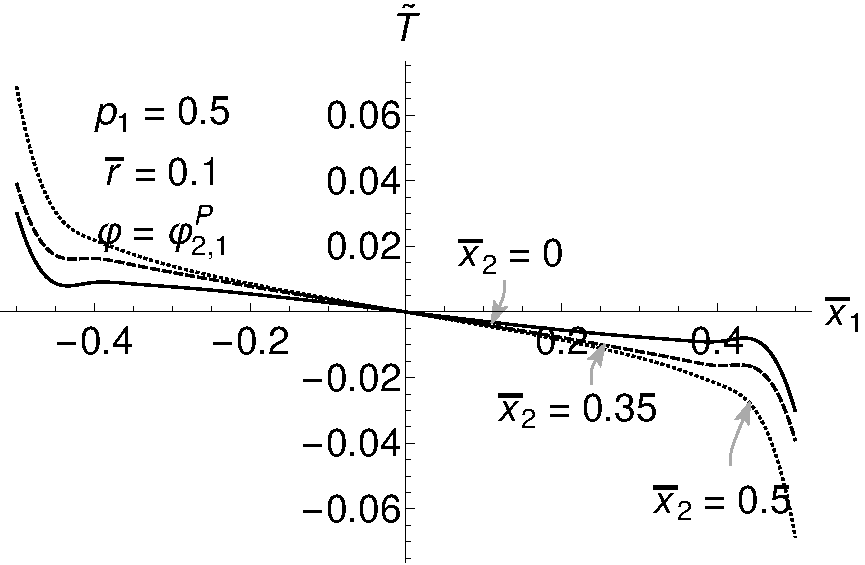
\includegraphics[width=\linewidth]{pics/TVarX2.pdf} \\ а)
    \end{minipage}
    \hfill
    \begin{minipage}[b][][b]{0.49\linewidth}\centering
        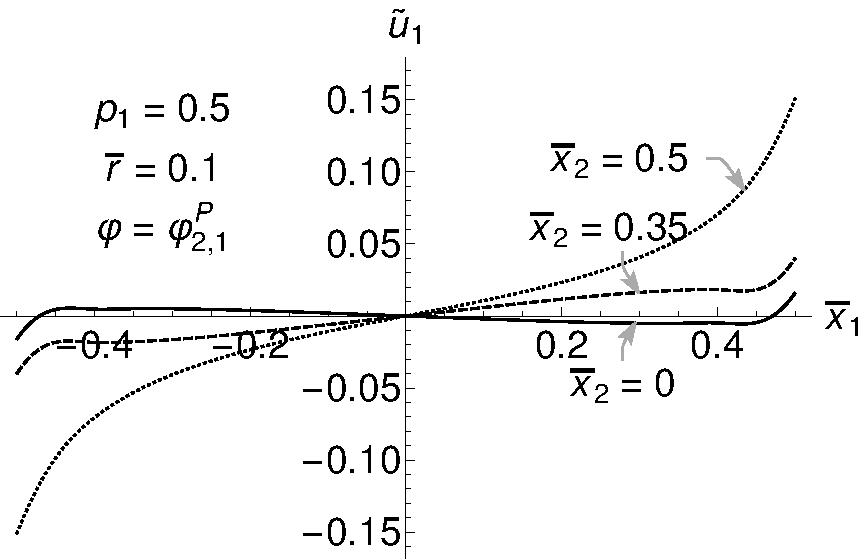
\includegraphics[width=\linewidth]{pics/U1VarX2.pdf} \\ б)
    \end{minipage}
    \caption{Нормированная разница решений в разных сечениях}
    \label{fig:VariationX2}
\end{figure}

Помимо уже рассмотренного, решения в нелокальной постановке также обладают и другими интересными особенностями. Например, в отличие от классического решения, компонента теплового потока $\overline{q}_2$ не равна нулю вблизи границ, где задан ненулевой тепловой поток, причём, как показано на Рис.~\ref{fig:Flux2}, решения обладают симметрией и также зависят от основных параметров модели. В отличие от температуры, увеличение радиуса нелокальности $\overline{r}$ не влияет на величину отклонений, но увеличивает размах кромочного эффекта, который здесь характеризуется увеличением площади областей, окружённых линиями уровней. Внутри области и на свободных от условий границах компонента плотности теплового потока $\overline{q}_2$ равна нулю.

\begin{figure}[ht]
    \begin{minipage}[b][][b]{0.49\linewidth}\centering
        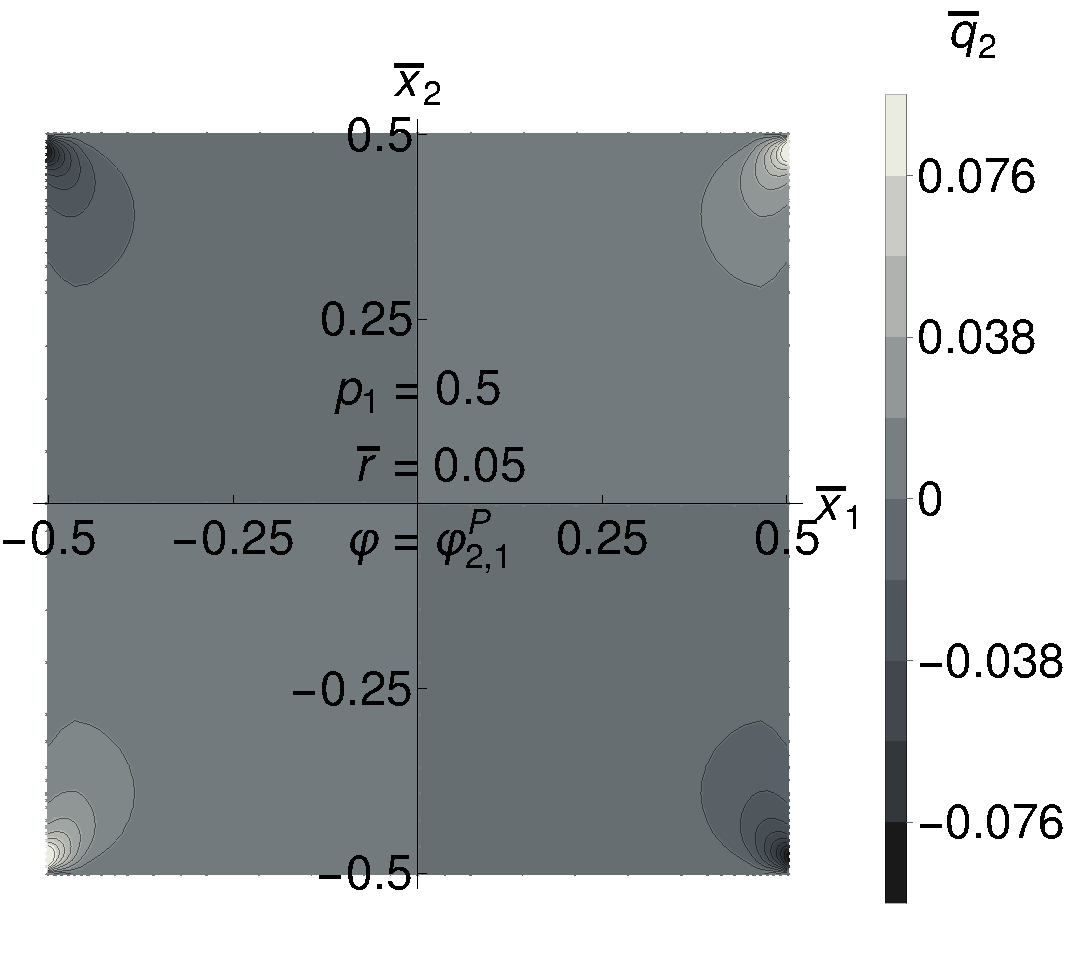
\includegraphics[width=\linewidth]{pics/Flux2R005.pdf} \\ а)
    \end{minipage}
    \hfill
    \begin{minipage}[b][][b]{0.49\linewidth}\centering
        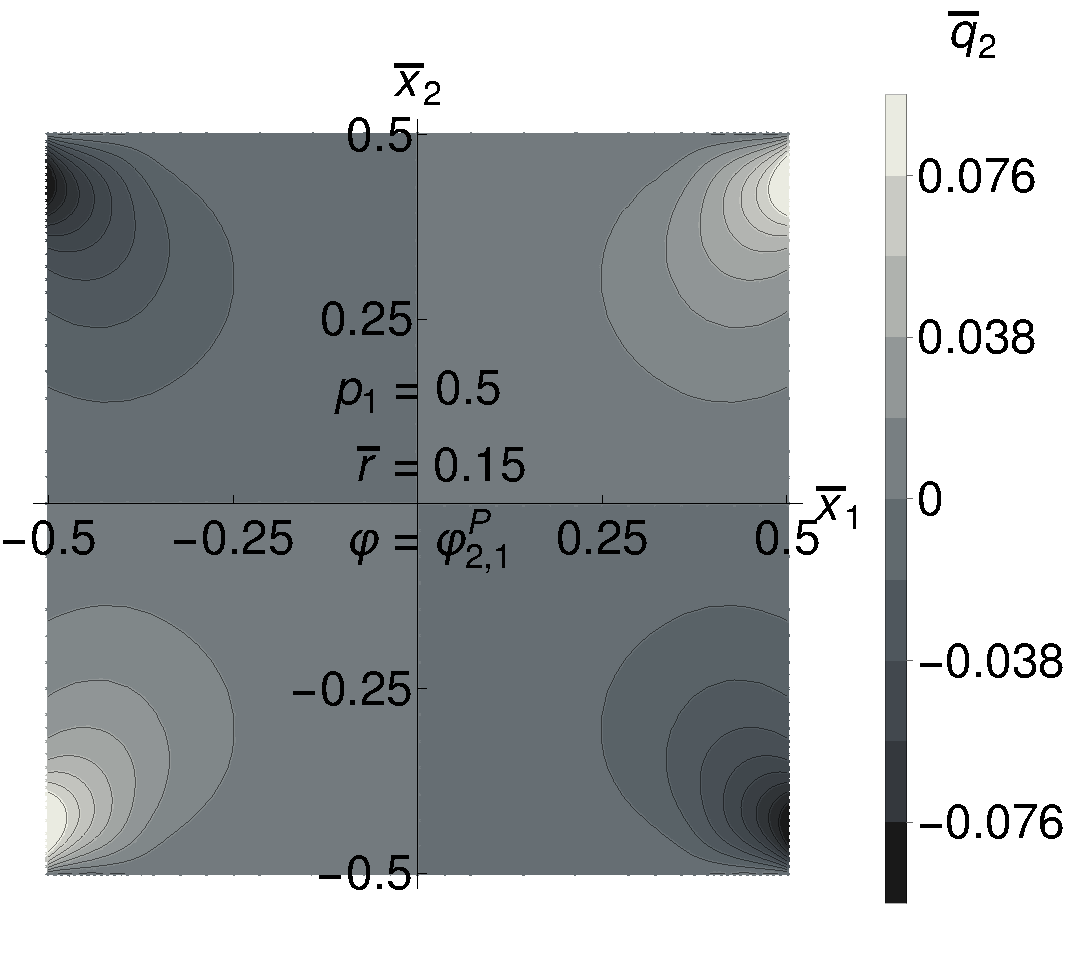
\includegraphics[width=\linewidth]{pics/Flux2R015.pdf} \\ б)
    \end{minipage}
    \caption{Распределение компоненты $\overline{q}_2$ при вариации $\overline{r}$}
    \label{fig:Flux2}
\end{figure}

Для уравнения равновесия в нелокальной постановке ненулевой становится компонента тензора напряжений $\overline{\sigma}_{12}$, а заодно и компонента тензора деформаций $\varepsilon_{12}$. Её распределение имеет более сложную, но при этом также симметричную форму и представлено на Рис.~\ref{fig:Sigma12}. Здесь, как и в случае с компонентой плотности теплового потока $\overline{q}_2$, вариация радиуса практически не оказывает влияния на максимальные значения напряжения и также увеличивает размах линий уровня. Отметим ещё, что на всех границах, включая те, где заданы нагружения, а также в центре области, значения $\overline{\sigma}_{12}$ равны нулю.

\begin{figure}[ht]
    \begin{minipage}[b][][b]{0.49\linewidth}\centering
        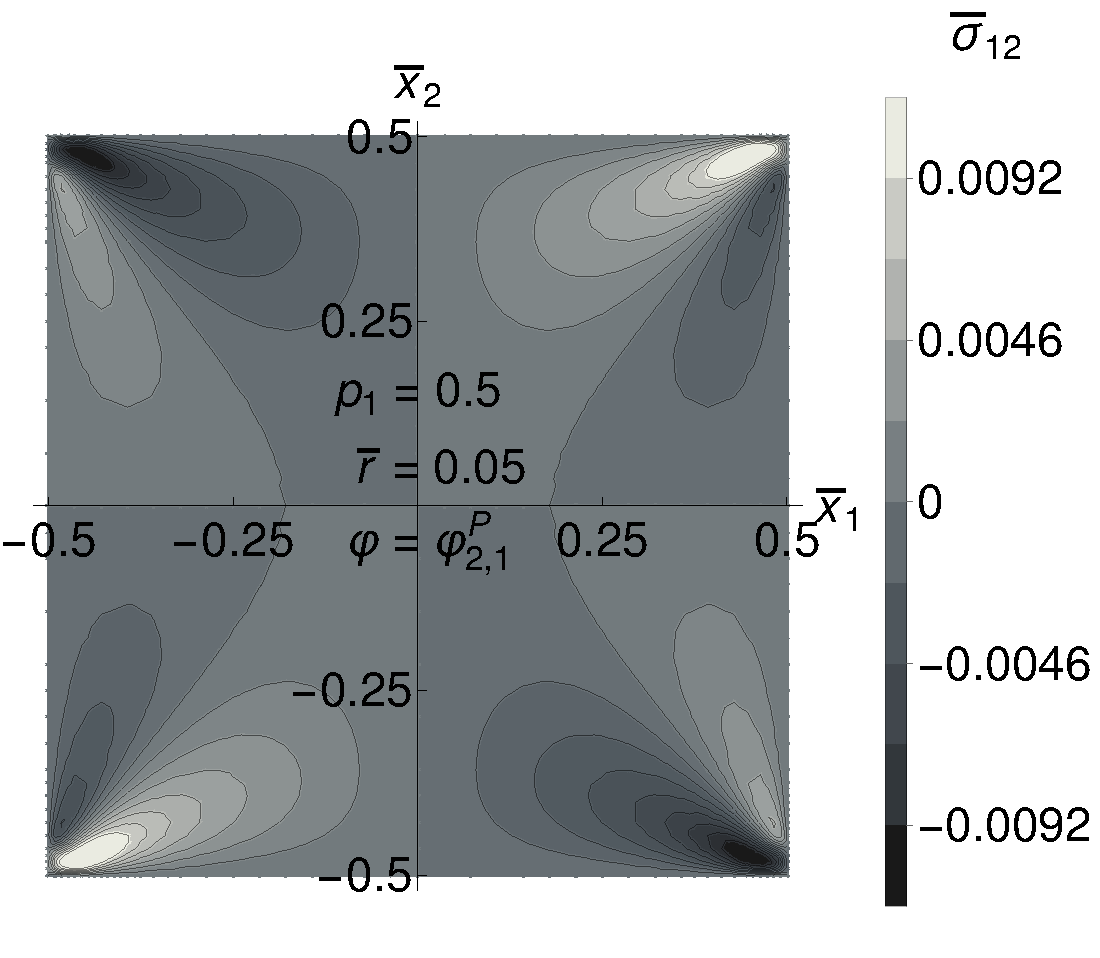
\includegraphics[width=\linewidth]{pics/Sigma12R005.pdf} \\ а)
    \end{minipage}
    \hfill
    \begin{minipage}[b][][b]{0.49\linewidth}\centering
        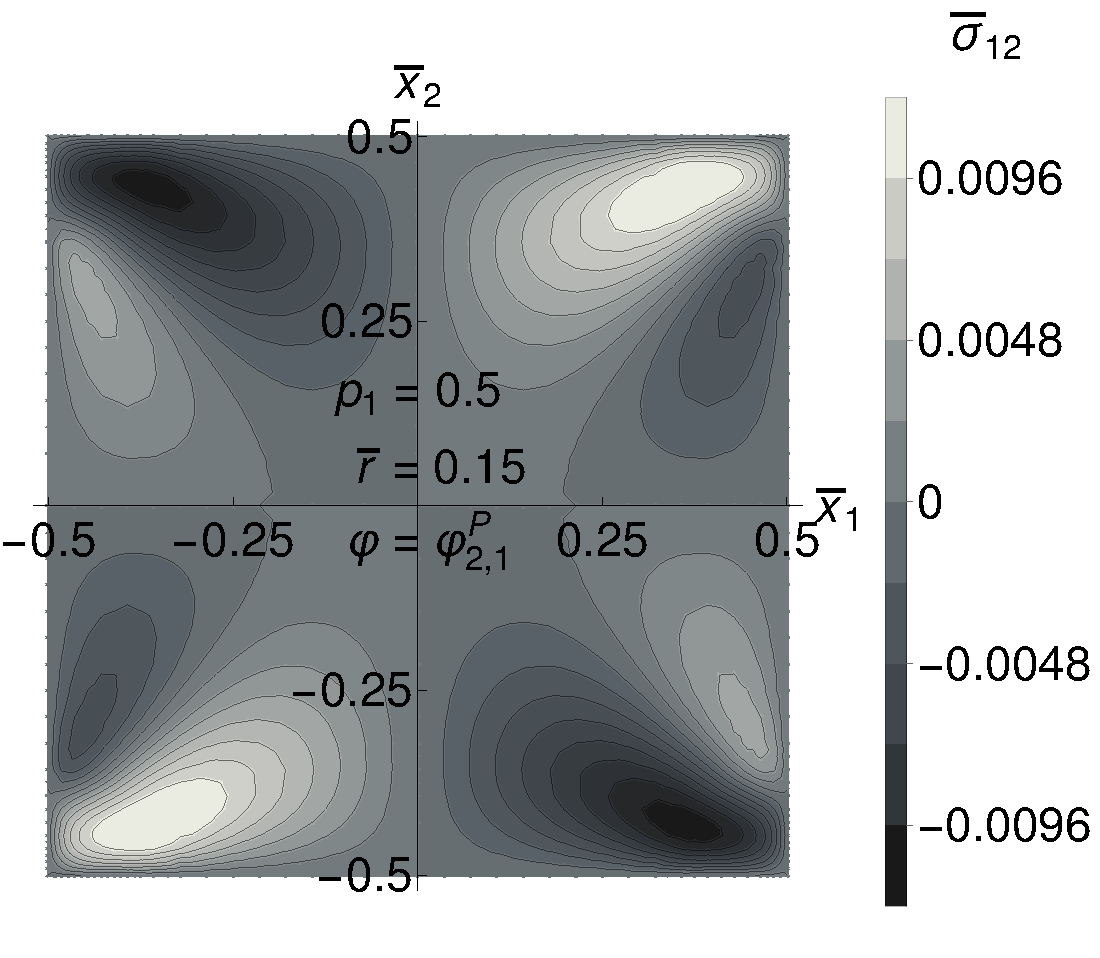
\includegraphics[width=\linewidth]{pics/Sigma12R015.pdf} \\ б)
    \end{minipage}
    \caption{Распределение компоненты $\overline{\sigma}_{12}$ при вариации $\overline{r}$}
    \label{fig:Sigma12}
\end{figure}

\section{Исследование функций нелокального влияния}\label{sec:ResultsAnalysis/KeyFeatures}

Изучим теперь влияние выбора функции нелокального влияния $\varphi$. Ранее уже были определены два параметрических семейства функций: полиномиальные $\varphi^P_{p,q}$ (\ref{eq:polynomialInfluence}) и экспоненциальные $\varphi^E_{p,q}$ (\ref{eq:exponentiallInfluence}). На их примере покажем как вариация основных параметров влияет на результаты решений. Не теряя общности исследования ограничимся решением только уравнения теплопроводности, но при этом будем сравнивать семейства функций между собой одновременно, так как их параметры, обозначенные одинаковыми символами, имеют одинаковый смысл. Рассматриваемую область и постановку задачи оставим той же, что уже была рассмотрена в предыдущем разделе.

Начнём исследование с вариации параметра $p$. Данный параметр отвечает за равномерность распределения функции влияния по заданной области $S'(\boldsymbol{x})$. Как показано на Рис.~\ref{fig:InfluenceVariationP}, отклонения решения растут вместе с параметром $p$ и достигают своего максимума, когда функция влияния вырождается в константу при $p \rightarrow \infty$. Здесь в качестве области нелокального влияния $S'(\overline{\boldsymbol{x}})$ был выбран круг с радиусом 0.1, поэтому для экспоненциального семейста функций был подобран и дисперсионный параметр нелокальности $\overline{r}$ при заданном квантиле $Q = 0.99$. Добавим ещё одно замечание, что для того, чтобы поведение экспоненциального семейства совпадало с полиномиальным, то есть увеличение параметра $p$ приводило к строгому увеличению отклонений, необходимо, чтобы параметр $p \geqslant n$.

\begin{figure}[ht]
    \begin{minipage}[b][][b]{0.49\linewidth}\centering
        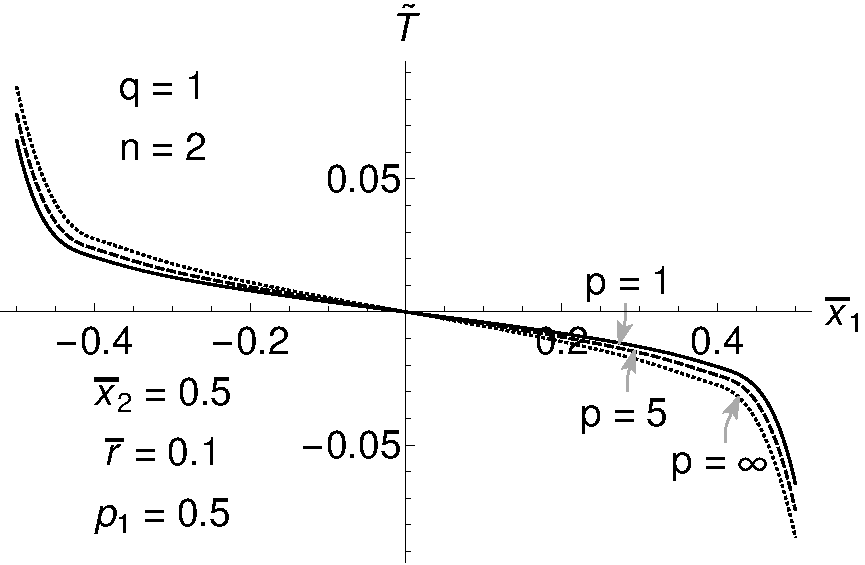
\includegraphics[width=\linewidth]{pics/TPolyInfluenceVariationP.pdf} \\ а)
    \end{minipage}
    \hfill
    \begin{minipage}[b][][b]{0.49\linewidth}\centering
        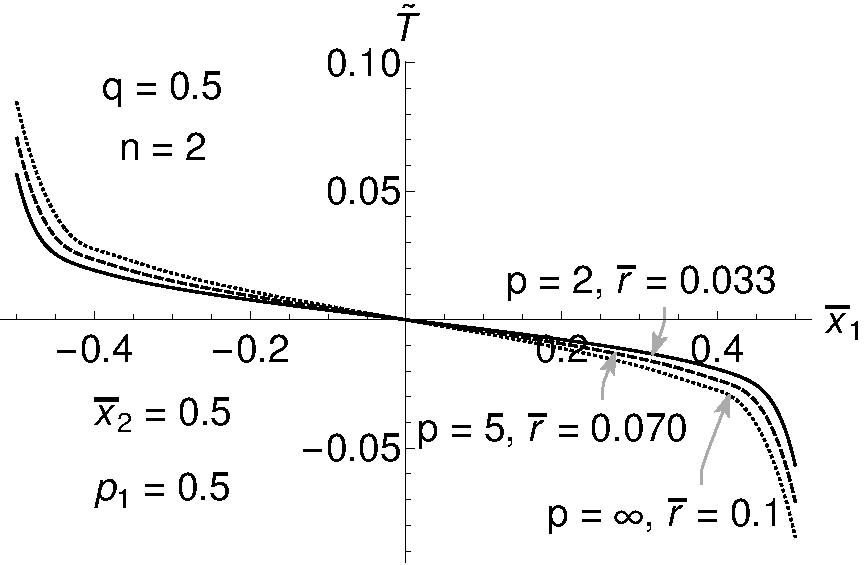
\includegraphics[width=\linewidth]{pics/TExpInfluenceVariationP.pdf} \\ б)
    \end{minipage}
    \caption{Вариация параметра $p$}
    \label{fig:InfluenceVariationP}
\end{figure}

Увеличение параметра $q$ концентрирует распределение функции нелокального влияния $\varphi$ в центре области $S'(\boldsymbol{x})$. Соответственно, при его увеличении отклонения решений относительно классического уменьшаются, что продемонстрировано на Рис.~\ref{fig:InfluenceVariationQ}. Здесь важно отметить, что для экспоненциальных функций дисперсионный параметр нелокальности $\overline{r}$ был выбран на основе функции с наименьшим значением параметра $q$, то есть для всех функций он совпадает. Сделано это по причине того, что данные параметры связаны между собой и если при изменении параметра $q$ подобрать подходящий под установленный квантиль $Q$ величину $\overline{r}$, распределения функций для всех $q$ будут совпадать.

\begin{figure}[ht]
    \begin{minipage}[b][][b]{0.49\linewidth}\centering
        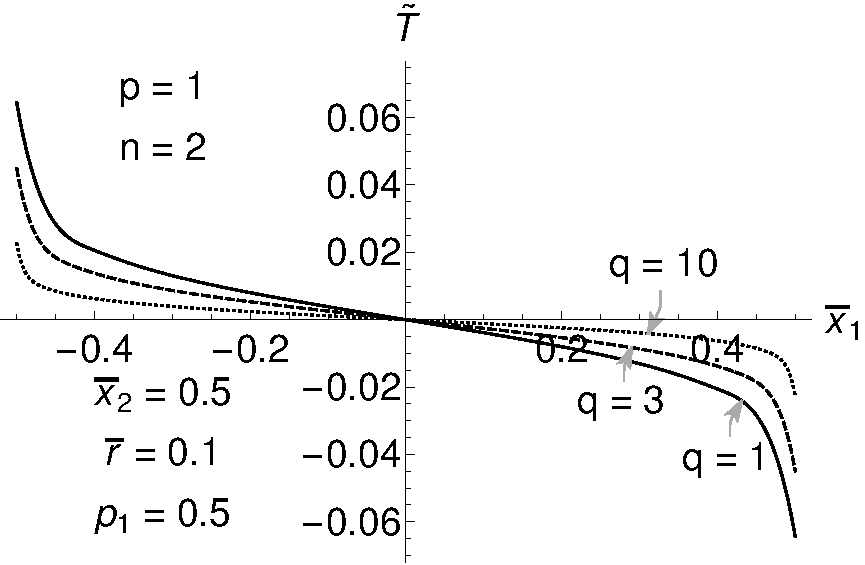
\includegraphics[width=\linewidth]{pics/TPolyInfluenceVariationQ.pdf} \\ а)
    \end{minipage}
    \hfill
    \begin{minipage}[b][][b]{0.49\linewidth}\centering
        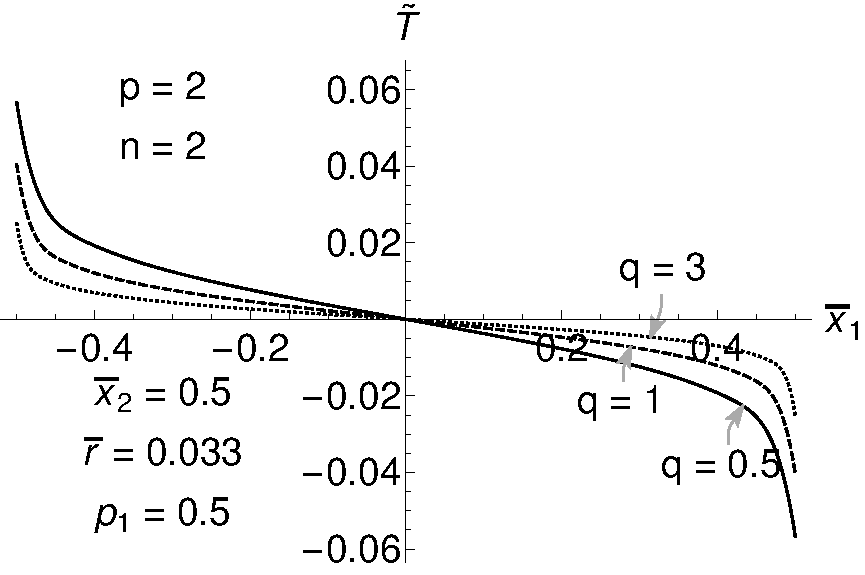
\includegraphics[width=\linewidth]{pics/TExpInfluenceVariationQ.pdf} \\ б)
    \end{minipage}
    \caption{Вариация параметра $q$}
    \label{fig:InfluenceVariationQ}
\end{figure}

Параметр $n$ является геометрическим, поэтому его изменение влияет на форму области $S'(\boldsymbol{x})$. Вместе с его увеличением увеличивается и покрываемая областью нелокального влияния площадь и, как показано на Рис.~\ref{fig:InfluenceVariationN}, отклонение решений. В силу независимости величины дисперсионного параметра $\overline{r}$ от параметра $n$ в уравнении (\ref{eq:quantil}), параметр $\overline{r}$ подбирался по правилу <<3 сигма>> на основе длины главной полуоси области $S'(\boldsymbol{x})$. Для экспоненциальных функций при заданных параметрах $p$ и $q$ влияние параметра $n$ становится несущественным, когда он больше $2$.

\begin{figure}[ht]
    \begin{minipage}[b][][b]{0.49\linewidth}\centering
        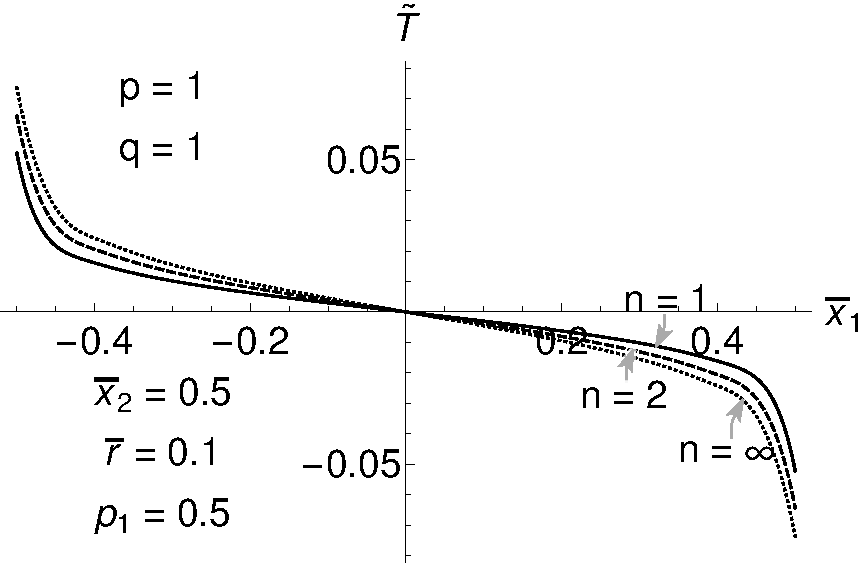
\includegraphics[width=\linewidth]{pics/TPolyInfluenceVariationN.pdf} \\ а)
    \end{minipage}
    \hfill
    \begin{minipage}[b][][b]{0.49\linewidth}\centering
        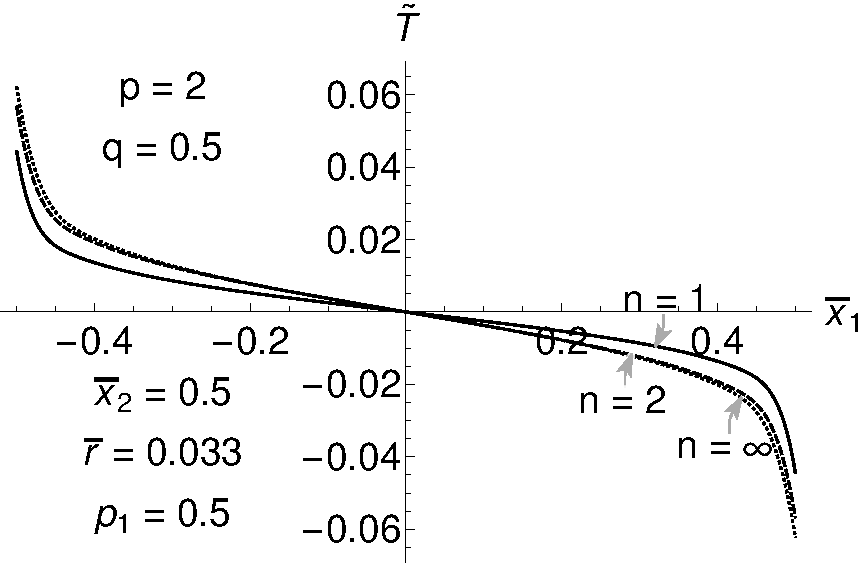
\includegraphics[width=\linewidth]{pics/TExpInfluenceVariationN.pdf} \\ б)
    \end{minipage}
    \caption{Вариация параметра $n$}
    \label{fig:InfluenceVariationN}
\end{figure}

Подведём некоторый промежуточный итог касательно выбора функции нелокального влияния $\varphi$. Было продемонстрировано, что её выбор может повлиять на степень отклонения решения, но качественных различий между решениями при различных параметрах функций нет. Также выбор семейства функций не оказывает существенного влияния на итоговые результаты. В связи с этими обстоятельствами, дальнейшие расчёты были проведены только с использованием квадратичных парабол $\varphi_{2,1}^P$ при $n = 2$, в силу того, что расчёты с использованием этой функции требуют наименьшего количества вычислительных ресурсов и этапы ассемблирования матрицы, вычисления тепловых потоков и напряжений происходят гораздо быстрее. Конечно, ещё меньше вычислительных операций требует функция $\varphi \equiv \text{const}$, но такая функция является предельной и не обладает свойством монотонного убывания из-за чего её использование формально является некорректным.

\section{Принципы Сен-Венана и стабильности теплового потока}\label{sec:ResultsAnalysis/SaintVenant}

Изучение свойств нелокальной теплопроводности и упругости следует начинать с простых задач, на примере которых можно исследовать основные принципы и положения присущие классическим моделям. К таким положениям можно отнести принцип стабильности теплового потока \cite{ThermalStability} и принцип Сен-Венана \cite{SaintVenant}, согласно которым любые интегрально эквивалентные возмущения поля являются локальными и вызывают одинаковые распределения поля вдали от точек приложения возмущения. В частности, для уравнения теплопроводности (\ref{eq:StationaryHeatEquation}) таким полем является поле плотности теплового потока $\boldsymbol{q}$, а для уравнения равновесия (\ref{eq:EquilibriumEquation}) --- поле \mbox{напряжений $\widehat{\boldsymbol{\sigma}}$.}

Для проверки этого высказывания проведём серию расчётов на прямоугольной области $S = \left\{ \boldsymbol{x} | -5 \leqslant x_1 \leqslant 5, -0.5 \leqslant x_2 \leqslant 0.5 \right\}$, с введённой на ней равномерной сеткой $S_h$ состоящей из $1500 \times 150$ элементов. Сформулируем граничные и интегральное условия для уравнения теплопроводности
\begin{gather*}
	\boldsymbol{n} \cdot \overline{\boldsymbol{q}} |_{\overline{x}_1 = -5} = f(\overline{x}_2),
	\quad
	\boldsymbol{n} \cdot \overline{\boldsymbol{q}} |_{\overline{x}_1 = 5} = -f(\overline{x}_2),
	\quad
	\iint\limits_S T dS = 0,
\end{gather*}
а также сформулируем граничные и геометрические условия для уравнения равновесия
\begin{gather*}
	n_j \overline{\sigma}_{j1} |_{\overline{x}_1 = -5} = -f(\overline{x}_2),
	\quad
	n_j \overline{\sigma}_{j1} |_{\overline{x}_1 = 5} = f(\overline{x}_2),
	\quad
	\overline{u}_1 |_{\overline{x}_1 = 0} = 0,
	\quad
	\overline{u}_2 |_{\overline{x}_2 = 0} = 0,
\end{gather*}
где $f$ --- функция задающая возмущение поля. Будем рассматривать три интегрально эквивалентных варианта возмущения
\begin{gather*}
	f_1 (x) = 1,
	\quad
	f_2 (x) = 2 - 4 |x|,
	\quad
	f_3 (x) = 4 |x|,
\end{gather*}
приложение которых, в виде теплового потока и давления заданных на левой и правой границах области $S$, изображено на Рис.~\ref{fig:SaintVenantLoads}.

\begin{figure}[ht]
    \begin{minipage}[b][][b]{0.49\linewidth}\centering
        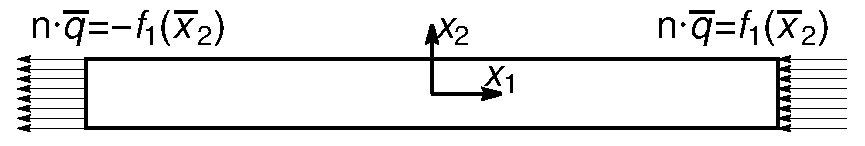
\includegraphics[width=\linewidth]{pics/RectangleFluxF1.pdf} \\ а)
        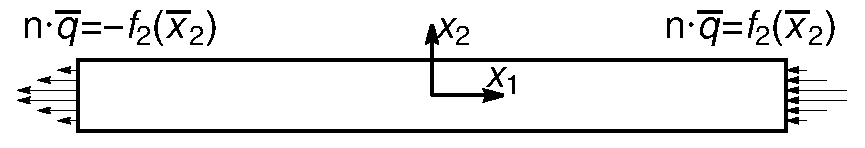
\includegraphics[width=\linewidth]{pics/RectangleFluxF2.pdf} \\ в)
        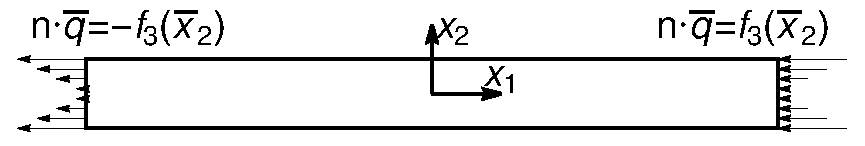
\includegraphics[width=\linewidth]{pics/RectangleFluxF3.pdf} \\ д)
    \end{minipage}
    \hfill
    \begin{minipage}[b][][b]{0.49\linewidth}\centering
        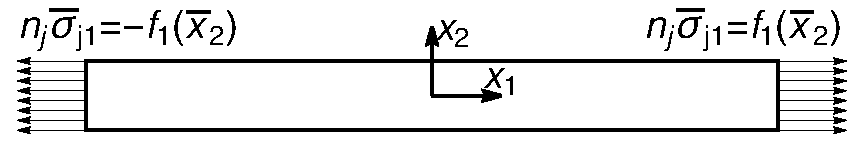
\includegraphics[width=\linewidth]{pics/RectangleStressF1.pdf} \\ б)
        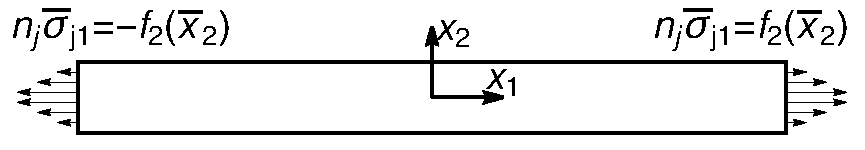
\includegraphics[width=\linewidth]{pics/RectangleStressF2.pdf} \\ г)
        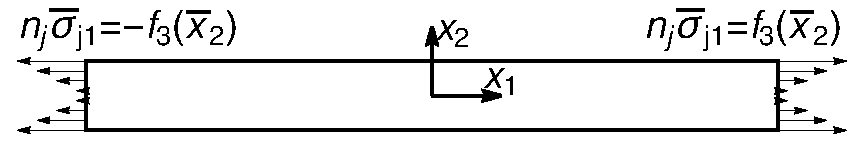
\includegraphics[width=\linewidth]{pics/RectangleStressF3.pdf} \\ е)
    \end{minipage}
    \caption{Тепловые (а, в, д) и механические (б, г, е) нагружения, прикладываемые к пластине на левой и правой границах}
    \label{fig:SaintVenantLoads}
\end{figure}

Вначале рассмотрим распределение компоненты теплового потока $\overline{q}_1$ в локальном и нелокальном контекстах. Для этого на Рис.~\ref{fig:FluxStability} рассмотрим сечения $\overline{x}_2 = 0$ и $\overline{x}_2 = 0.5$, где можем увидеть, что несмотря на различные тепловые потоки подведённые к левой и правой границам, при удалении от точек приложения потоки сливаются в единую поверхность, которая в локальном случае является плоскостью $\overline{q}_1 = 1$, а в нелокальном представляет более сложную поверхность.

\begin{figure}[ht]
    \begin{minipage}[b][][b]{0.49\linewidth}\centering
        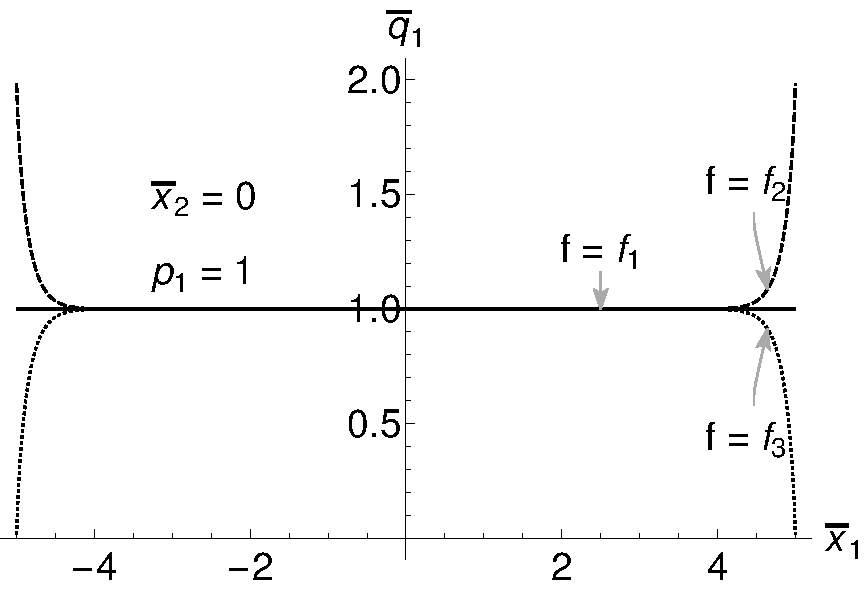
\includegraphics[width=\linewidth]{pics/FluxStabilityX0P1.pdf} \\ а)
        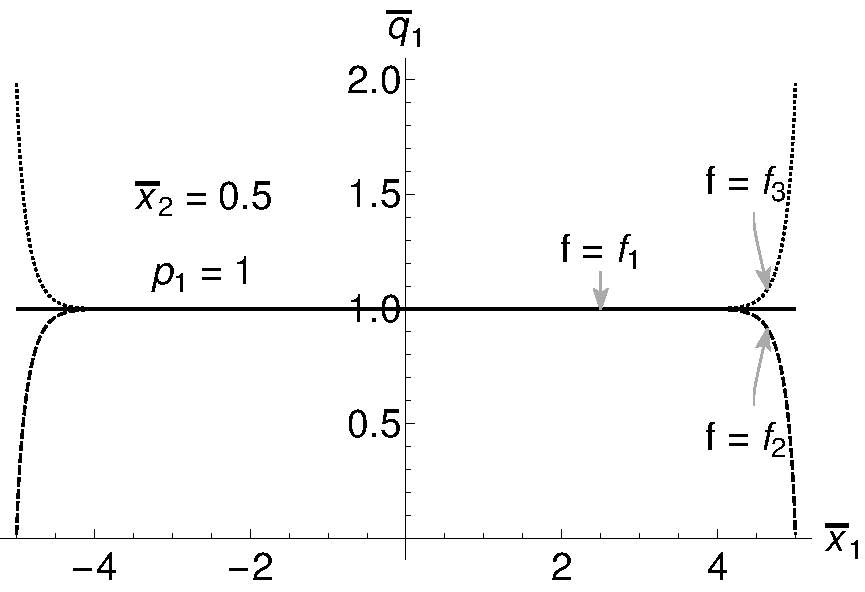
\includegraphics[width=\linewidth]{pics/FluxStabilityX05P1.pdf} \\ в)
    \end{minipage}
    \hfill
    \begin{minipage}[b][][b]{0.49\linewidth}\centering
        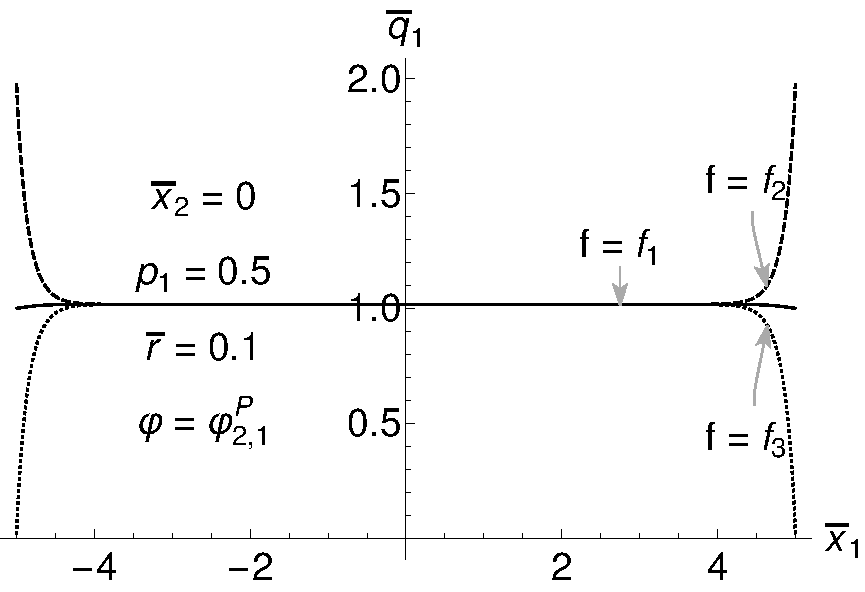
\includegraphics[width=\linewidth]{pics/FluxStabilityX0P05.pdf} \\ б)
        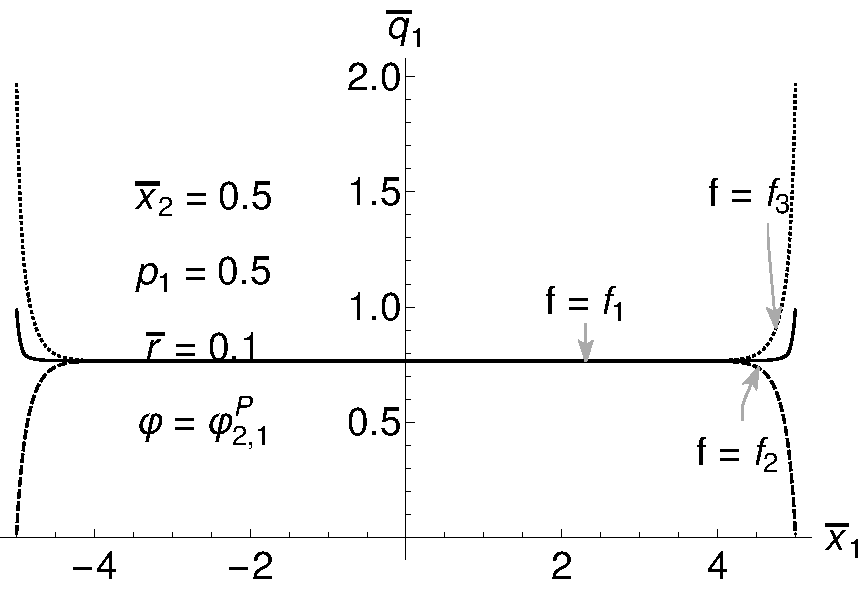
\includegraphics[width=\linewidth]{pics/FluxStabilityX05P05.pdf} \\ г)
    \end{minipage}
    \caption{Распределение компоненты плотности теплового потока $\overline{q}_1$ в сечениях (а, б) $\overline{x}_2 = 0$ и (в, г) $\overline{x}_2 = 0.5$ в (а, в) локальном и (б, г) нелокальном случаях}
    \label{fig:FluxStability}
\end{figure}

Теперь рассмотрим распределение компоненты тензора напряжений $\overline{\sigma}_{11}$. Здесь аналогично ранее рассмотренной компоненте плотности теплового потока $\overline{q}_1$ решения сливаются в общую поверхность, которая, как и в предыдущем случае, в локальной постановке является плоскостью $\overline{\sigma}_{11} = 1$, а в нелокальной представляет некоторую поверхность. На Рис.~\ref{fig:SaintVenant} представлены распределения компоненты тензора напряжений $\overline{\sigma}_{11}$ в сечениях $\overline{x}_2 = 0$ и $\overline{x}_2 = 0.5$ в локальной и нелокальной постановках.

\begin{figure}[ht]
    \begin{minipage}[b][][b]{0.49\linewidth}\centering
        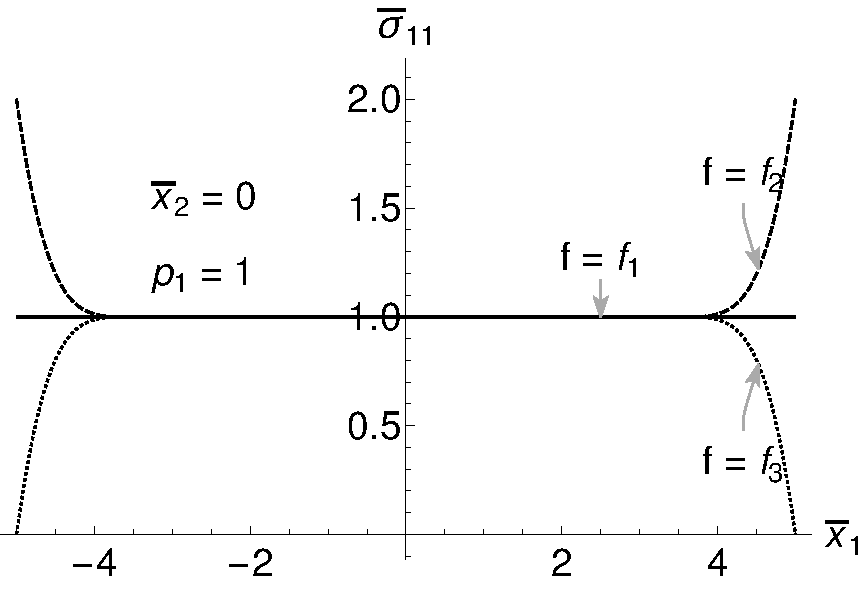
\includegraphics[width=\linewidth]{pics/SaintVenantX0P1.pdf} \\ а)
        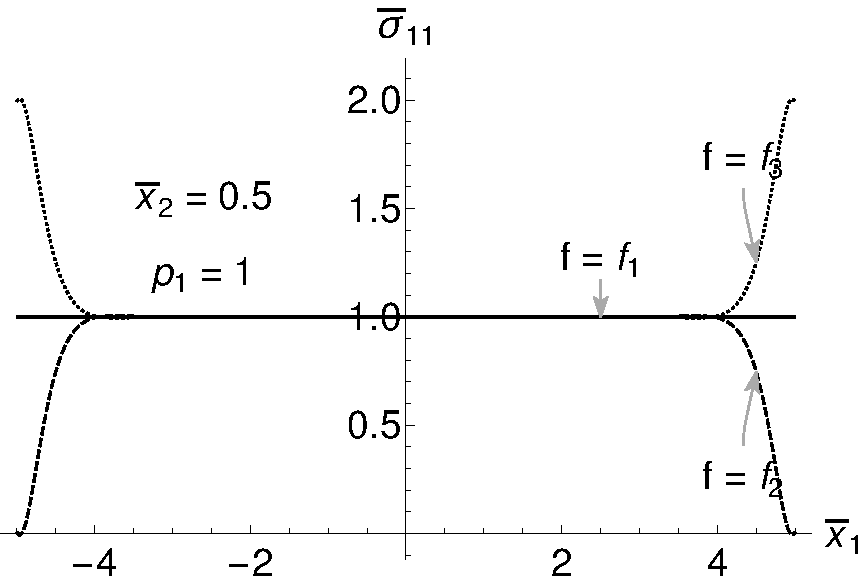
\includegraphics[width=\linewidth]{pics/SaintVenantX05P1.pdf} \\ в)
    \end{minipage}
    \hfill
    \begin{minipage}[b][][b]{0.49\linewidth}\centering
        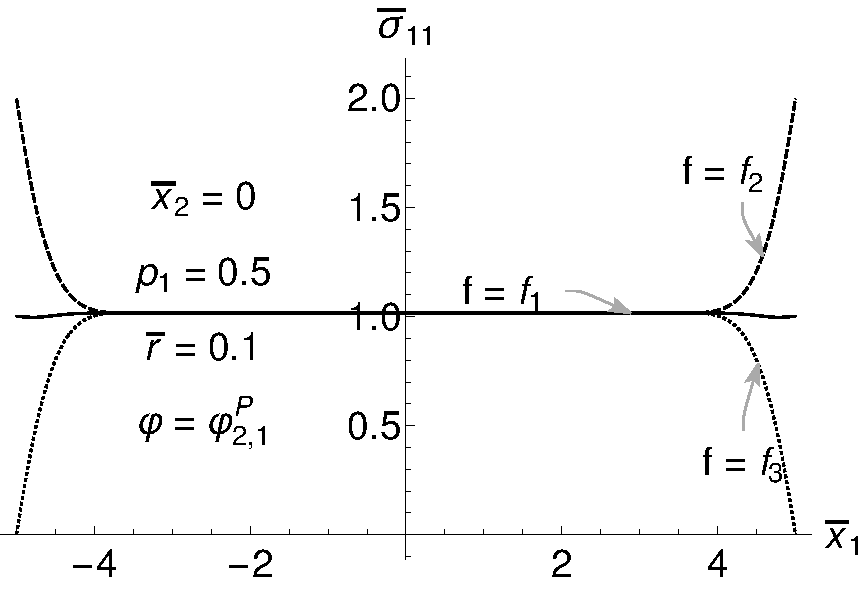
\includegraphics[width=\linewidth]{pics/SaintVenantX0P05.pdf} \\ б)
        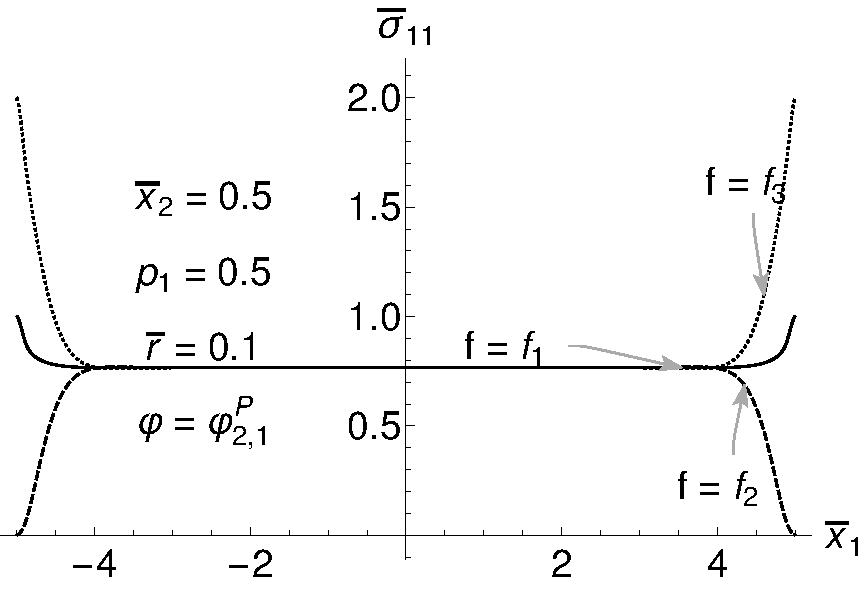
\includegraphics[width=\linewidth]{pics/SaintVenantX05P05.pdf} \\ г)
    \end{minipage}
    \caption{Распределение компоненты тензора напряжений $\overline{\sigma}_{11}$ в сечениях (а, б) $\overline{x}_2 = 0$ и (в, г) $\overline{x}_2 = 0.5$ в (а, в) локальном и (б, г) нелокальном случаях}
    \label{fig:SaintVenant}
\end{figure}

Рис.~\ref{fig:FluxStability} и \ref{fig:SaintVenant} имеют похожие кривые, однако, стабилизация теплового потока происходит заметно быстрее стабилизации напряжений. Для иллюстрации, представленной на Рис.~\ref{fig:StabilityLog10}, прологарифмируем разницу решений полученных при нагружениях с использованием функций $f_1$ и $f_2$, где для обобщения обозначений по оси ординат решения будем обозначать символами  $\mathcal{S}_1$ и $\mathcal{S}_2$ соответственно. В полученных распределениях можем увидеть, что локальные и нелокальные решения имеют одинаковый характер сходимости, но в центре области расхождения между ними начинают нарастать, причём в случае тепловых потоков разница достигает около двух порядков, однако, учитывая порядок величин, такое расхождение можно связать с погрешностями вычислений. Также стоит отметить, что стабилизация теплового потока происходит монотонно, в то время как стабилизация напряжений имеет осцилирующий характер, что можно понять по изломам графика, где происходит пересечение кривых.

\begin{figure}[ht]
    \begin{minipage}[b][][b]{0.49\linewidth}\centering
        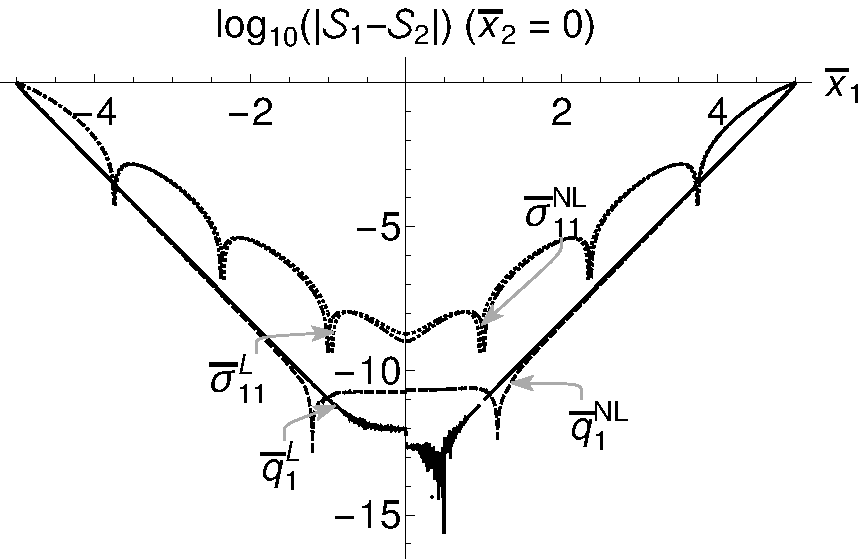
\includegraphics[width=\linewidth]{pics/StabilityLogX0.pdf} \\ а)
    \end{minipage}
    \hfill
    \begin{minipage}[b][][b]{0.49\linewidth}\centering
        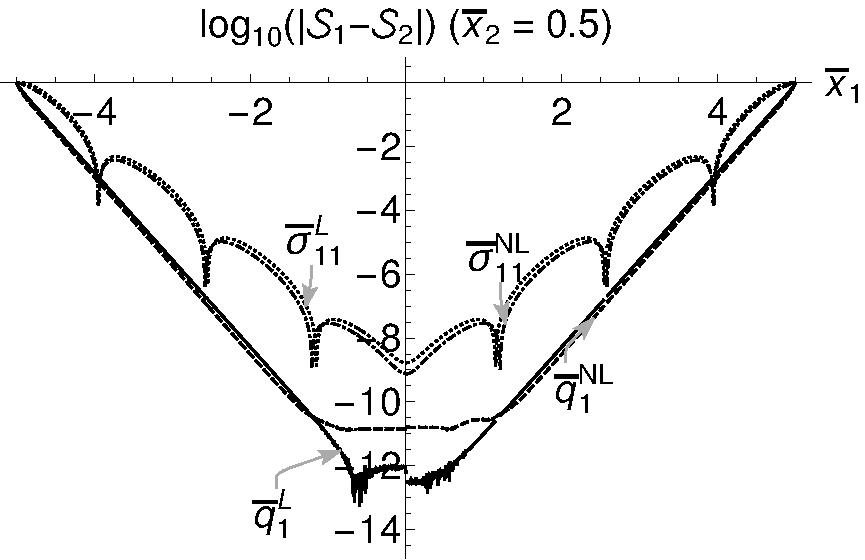
\includegraphics[width=\linewidth]{pics/StabilityLogX05.pdf} \\ б)
    \end{minipage}
    \caption{Логарифмическая разность решений при различных нагружениях в сечениях (a) $\overline{x}_2 = 0$ и (б) $\overline{x}_2 = 0.5$}
    \label{fig:StabilityLog10}
\end{figure}

Теперь рассмотрим сечение вдоль оси $\text{O}\overline{x}_2$. В этом сечении решения обладают кромочным эффектом, который проявляется в снижении уровня рассматриваемой величины на свободных границах области и компенсирующим это снижение повышении этой величины в центре. Вариация радиуса нелокальности $\overline{r}$ увеличивает размах кромочного эффекта, а вариация весового параметра $p_1$ влияет на величину отклонения. При этом заметим, что при фиксированном радиусе нелокальности $\overline{r}$ все решения, при различных значениях параметра $p_1$, пересекаются в общих точках. В силу того, что графики компоненты теплового потока $\overline{q}_1$ и компоненты напряжений $\overline{\sigma}_{11}$ в этом сечении визуально не отличаются, изобразим их на общем Рис.~\ref{fig:SaintVenantVariation}, указав по оси ординат обобщающий их символ $\mathcal{S}$.

\begin{figure}[ht]
    \begin{minipage}[b][][b]{0.49\linewidth}\centering
        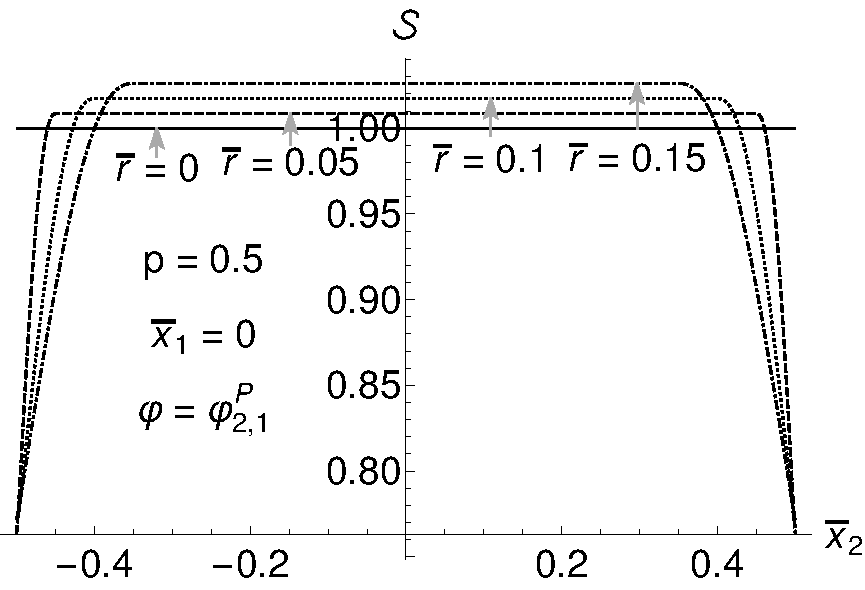
\includegraphics[width=\linewidth]{pics/HeatFluxStabilityVariationR.pdf} \\ а)
    \end{minipage}
    \hfill
    \begin{minipage}[b][][b]{0.49\linewidth}\centering
        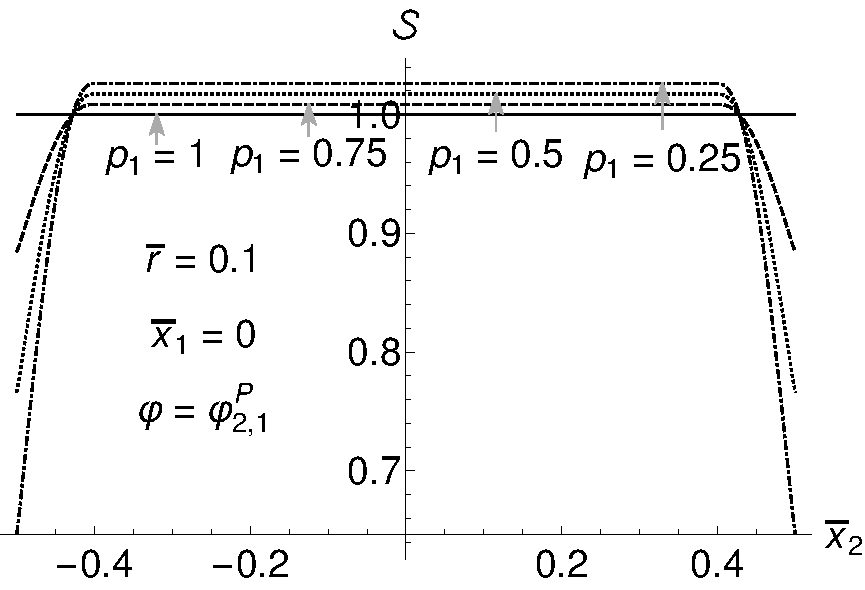
\includegraphics[width=\linewidth]{pics/HeatFluxStabilityVariationP1.pdf} \\ б)
    \end{minipage}
    \caption{Распределение компоненты теплового потока $\overline{q}_1$ и компоненты тензора напряжений $\overline{\sigma}_{11}$ в сечении $\overline{x}_1 = 0$ при вариации (а) $\overline{r}$ и (б) $p_1$}
    \label{fig:SaintVenantVariation}
\end{figure}

Во всех сечениях равнодействующие компоненты теплового потока $\overline{q}_1$ и напряжения $\overline{\sigma}_{11}$ сохраняются и равны приложенным нагружениям:
\begin{gather*}
	\int\limits_{-0.5}^{0.5} \overline{q}_1 d\overline{x}_2 = 
	\int\limits_{-0.5}^{0.5} f_i (\overline{x}_2) d\overline{x}_2,
	\quad
	\int\limits_{-0.5}^{0.5} \overline{\sigma}_{11} d\overline{x}_2 = 
	\int\limits_{-0.5}^{0.5} f_i (\overline{x}_2) d\overline{x}_2,
	\quad	
	i = \overline{1,3}.
\end{gather*}
Это свидетельствует о выполнении принципов стабильности теплового потока и Сен-Венана, а также сохранении балансных соотношений.

\section{Растяжение пластины со ступенчатым переходом}\label{sec:ResultsAnalysis/TShape}

Большой интерес представляет поведение модели на областях с сингулярными точками, где решения стремятся к бесконечности при дроблении сетки. К таким областям относятся области со ступенчатыми переходами, часто возникающими в различных конутрукционных деталях. Для изучения особенностей будет достаточно одного перехода, поэтому рассмотрим простейшую Т-образную область $S$ заключённую в единичный квадрат $\overline{S} = \left\{ \boldsymbol{x} \ | \ 0 \leqslant x_1, x_2 \leqslant 1 \right\}$, изображённую на Рис.~\ref{fig:TArea} с интересующими нас сечениями AB, CD, EF и GH. Приложим следующие граничные и геометрические условия
\begin{gather*}
	n_j \overline{\sigma}_{j2} |_{\overline{x}_2 = 0} = -1,
	\quad
	\overline{u}_2 |_{\overline{x}_2 = 1} = 0,
	\quad
	\overline{u}_1 |_{\overline{x}_1 = 0.5} = 0.
\end{gather*}
Решение будем искать на равномерной сетке $S_h$ с характерным размером элементов $h = 1/300$.

\begin{figure}[ht]
    \centerfloat{
        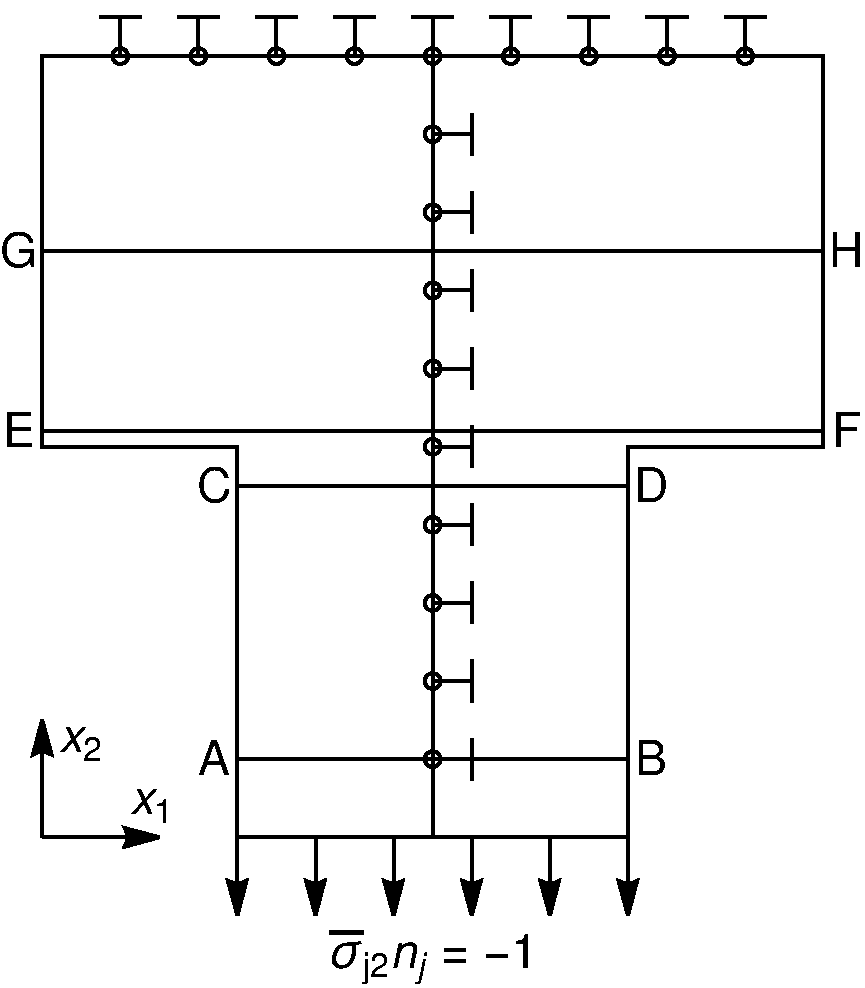
\includegraphics[width=0.5\textwidth]{pics/TArea.pdf}
    }
    \caption{Т-образная область с приложенной нагрузкой}
    \label{fig:TArea}
\end{figure}

Распределение полей компоненты деформации $\varepsilon_{22}$ в локальном и нелокальном случаях при различных радиусах нелокальности $\overline{r}$ представлены на Рис.~\ref{fig:TEpsilon}. В нелокальном случае линии уровня изменяют свой характер вблизи границ области, особенно в области ступенчатого перехода, где помимо прочих искажений, можем наблюдать увеличение деформаций, причём как положительных, так и отрицательных. Линии уровня в зонах с отрицательной деформацией становятся более выраженными и их размах увеличивается вместе с радиусом нелокальности $\overline{r}$. В отличие от классического случая, в точках приложения нагружения поле деформации $\varepsilon_{22}$ неравномерно, несмотря на равномерный характер нагружения, что характеризуется повышенными значениями деформации в нижних углах нижней части области. Вблизи точек закрепления линии уровня терпят излом, характеризующийся резкой сменой направления линии, которая по итогу, в отличие от классического случая, выходит на границу области не под прямым углом. Крутизна излома уменьшается при увеличении радиуса нелокальности, а расстояние от границы до излома увеличивается.

\begin{figure}[ht]
    \begin{minipage}[b][][b]{0.49\linewidth}\centering
        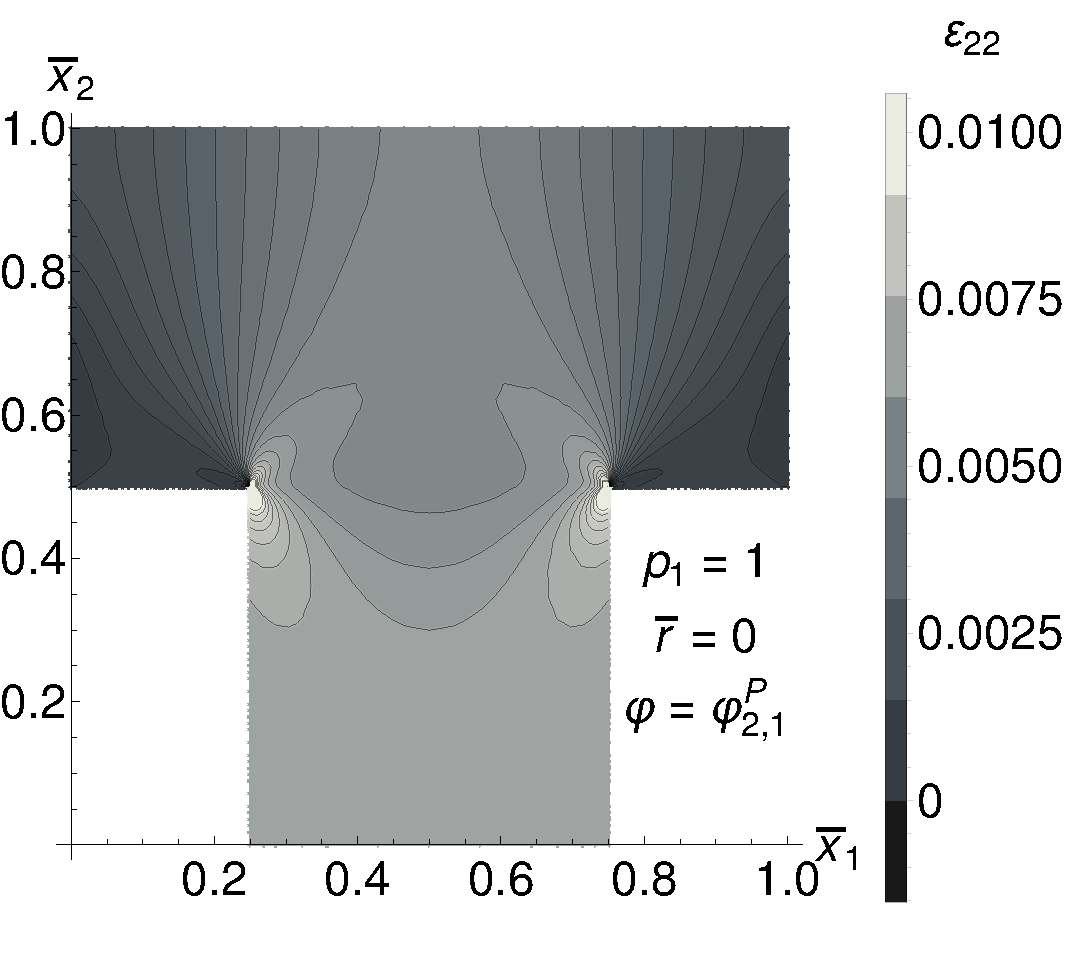
\includegraphics[width=\linewidth]{pics/TEpsR0.pdf} \\ а)
        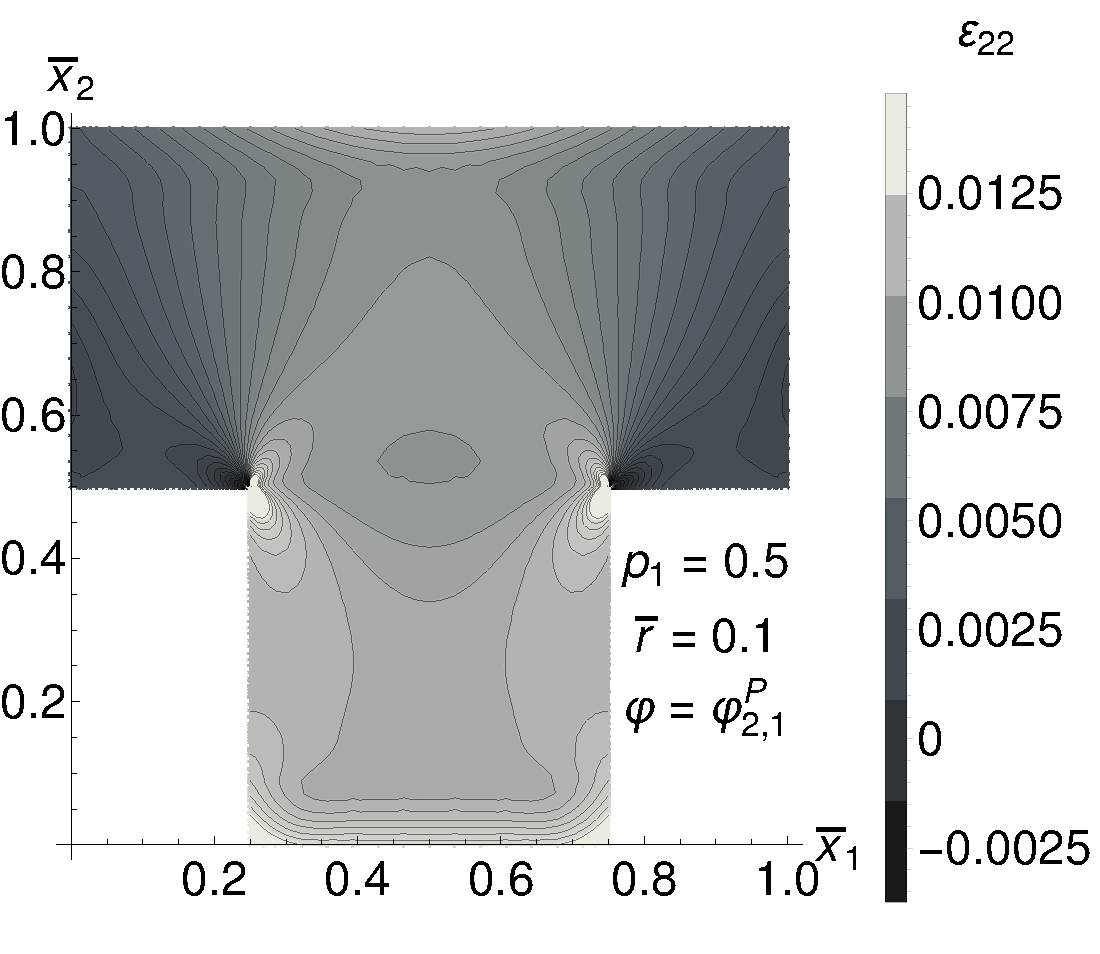
\includegraphics[width=\linewidth]{pics/TEpsR01.pdf} \\ в)
    \end{minipage}
    \hfill
    \begin{minipage}[b][][b]{0.49\linewidth}\centering
        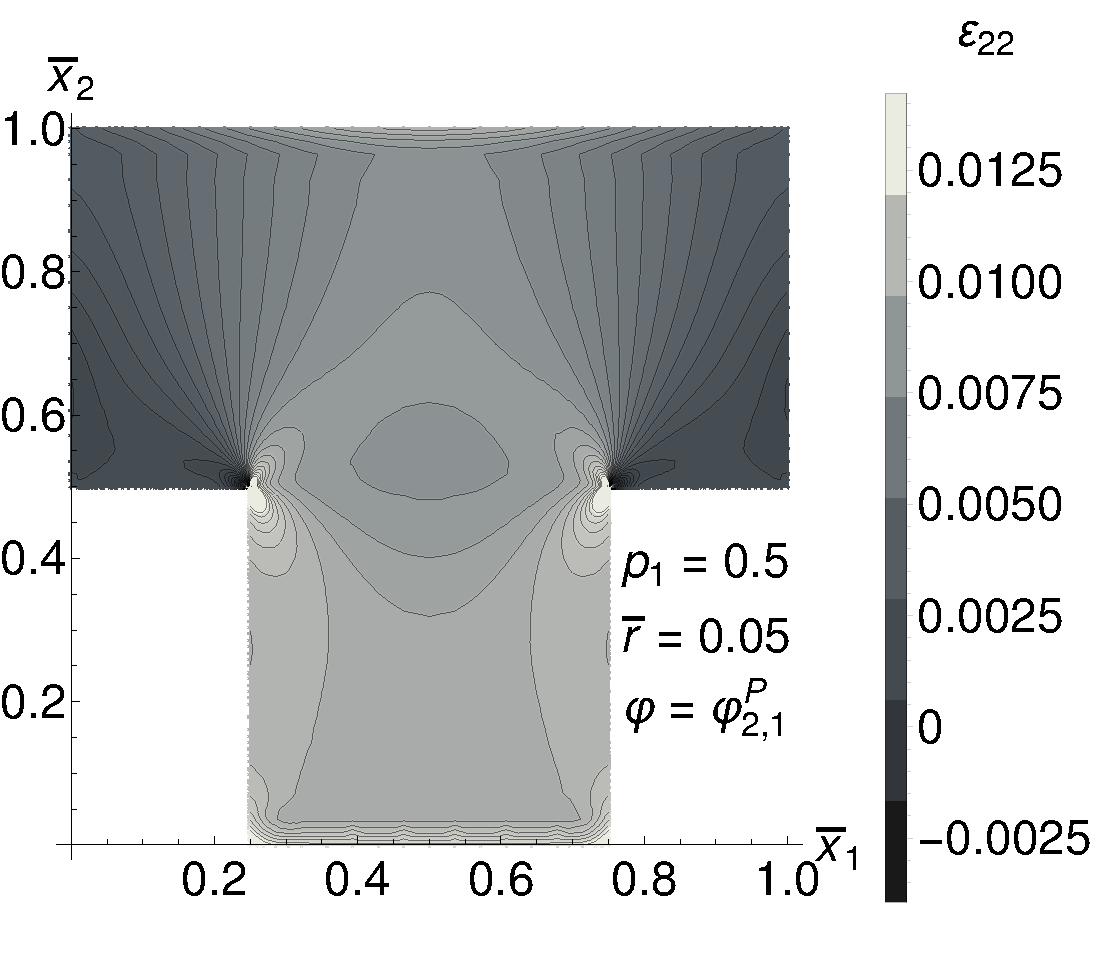
\includegraphics[width=\linewidth]{pics/TEpsR005.pdf} \\ б)
        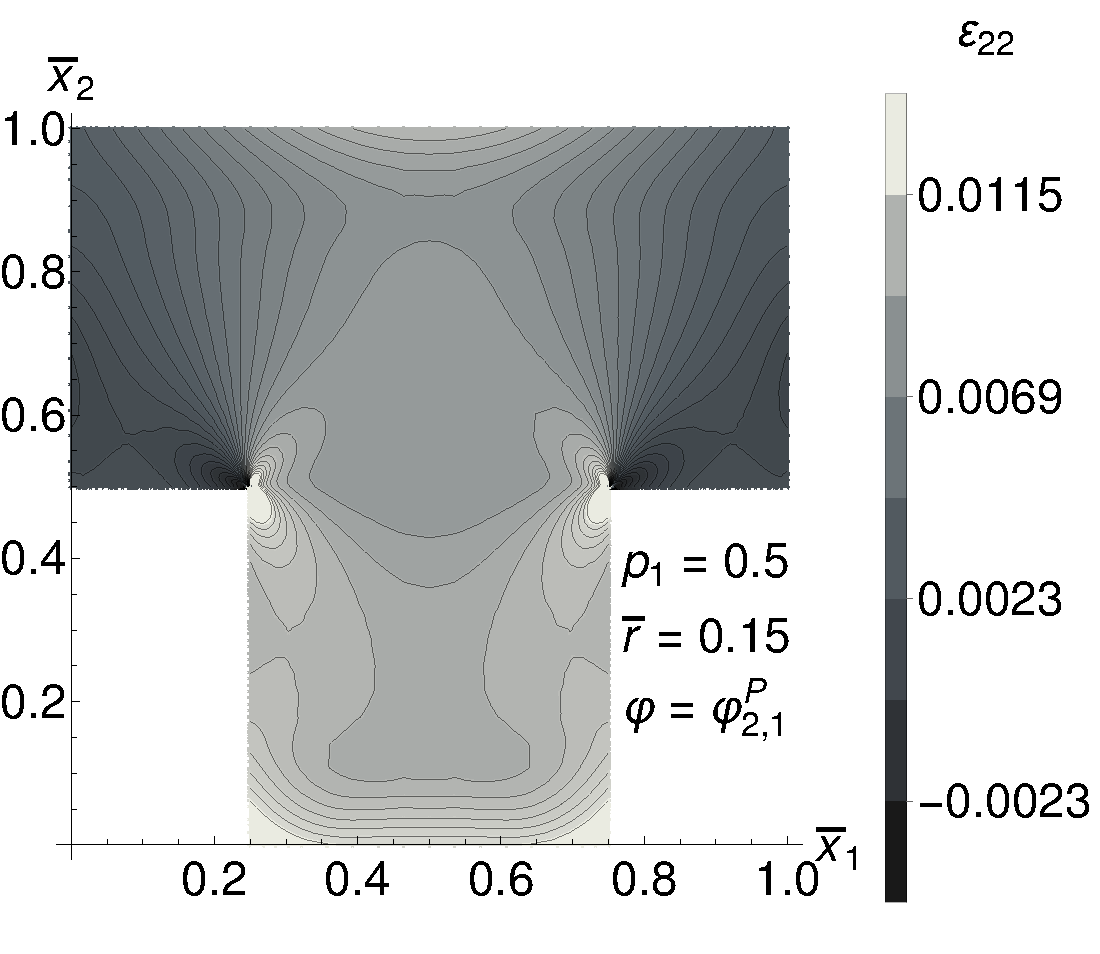
\includegraphics[width=\linewidth]{pics/TEpsR015.pdf} \\ г)
    \end{minipage}
    \caption{Распределение компоненты тензора деформации $\varepsilon_{22}$ при различных радиусах нелокальности $\overline{r}$}
    \label{fig:TEpsilon}
\end{figure}

Аналогичные распределения деформации в областях со ступенчатыми переходами были получены в результате серии экспериментов под руководством А.В.~Андреева с точным измерением деформаций на пластинах из оптически активных материалов \cite{Andreev}. Деформации измерялись в различных сечениях пластины с использованием 120 тензородатчиков с одинковым механическим сопротивлением. Также был использован альтернативный метод измерения деформации с использованием оптических приборов, где при помощи нанесённой на пластину сетки измерялись перемещения её узлов. При помощи закона Гука и экспериментальных данных о деформациях были определены напряжения и найдены их равнодействующие в сечениях. В работе А.В.~Андреева было показано, что на участке, отстоящем от ступенчатого перехода примерно на четверть ширины ступени наблюдались наиболее резкие изменения полей деформации и напряжений. Кроме того, в результате экспериментов было установлено, что равнодействующая напряжений, расчитанная по формуле
\begin{gather*}
	\overline{\sigma}_{22}^* = \int\limits_{l_1}^{l_2} \overline{\sigma}_{22} d \overline{x}_1,
\end{gather*}
в сечениях, достаточно удалённых от ступенчатого перехода, равна приложенной нагрузке, а результирующие напряжения в сечениях близких к ступенчатому переходу, оказались в среднем на 30\% меньше приложенного нагружения. Эффект сохранялся при различных значениях нагрузки, а также при двух предельных формах закона Гука, соответствующих плоскому деформированному и плоскому напряжённому состояниям. Объяснением подобного эффекта в работе А.В. Андреева вероятно является тот факт, что классическая теория упругости при расчёте напряжений не позволяет учесть структурных особенностей материала, что и привело к неправильной интерпретации полученных данных.
% Структурная анизотропия???

Действительно, если подставить значения деформации, представленные на Рис.~\ref{fig:TEpsilon}, в классический закон Гука, то можно получить результаты, похожие на те, что были описаны в эксперименте. Распределения результирующего напряжения $\overline{\sigma}_{22}^*$, представленные на Рис.~\ref{fig:ResultantStress22}, также демонстрируют некоторое снижение напряжения сразу после ступенчатого перехода, но не на 30\%, как это было описано в экспериментах. В нижней части области ситуация обратная, результирующее напряжение выше приложенной нагрузки, а в области перехода можем наблюдать резкий градиент. Максимум отклонения находится на нижней и верхней границах области. Отметим, что наибольший вклад на величину отклонения влизи границ области оказывает весовой параметр $p_1$, а на величину отклонения внутри области, а также на ширину отклонения, радиус нелокальности $\overline{r}$. При расчёте напряжений по формуле (\ref{eq:DuamelNeumann}) равнодействующая напряжений во всех сечениях равна постоянной, интегрально совпадающей с приложенной нагрузкой.

\begin{figure}[ht]
    \begin{minipage}[b][][b]{0.49\linewidth}\centering
        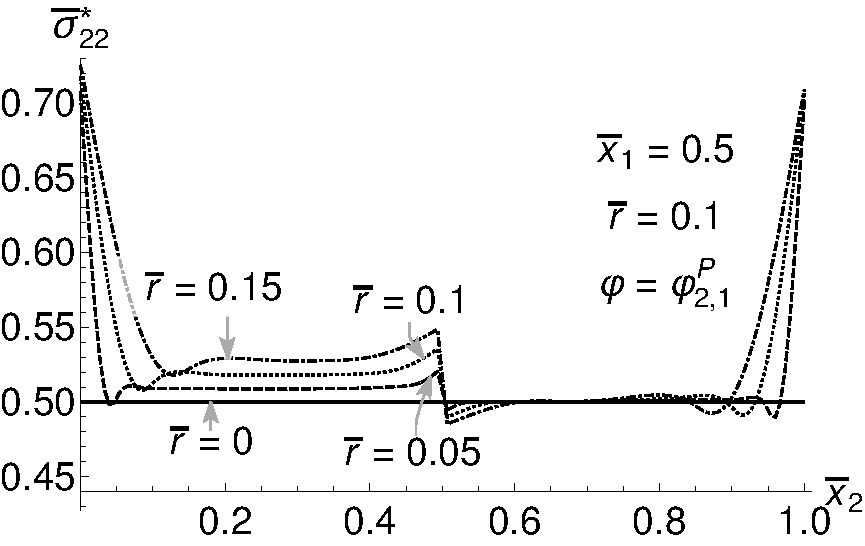
\includegraphics[width=\linewidth]{pics/ResultantStressVariationR.pdf} \\ а)
    \end{minipage}
    \hfill
    \begin{minipage}[b][][b]{0.49\linewidth}\centering
        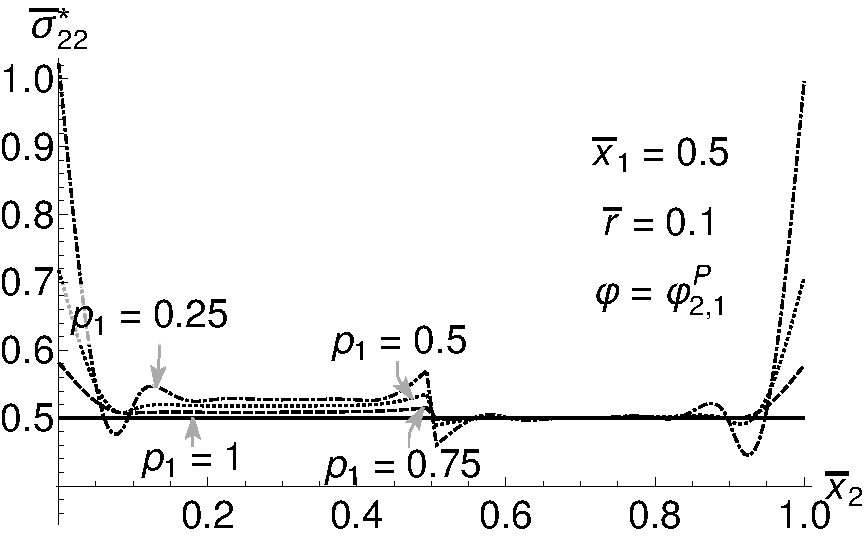
\includegraphics[width=\linewidth]{pics/ResultantStressVariationP1.pdf} \\ б)
    \end{minipage}
    \caption{Равнодействующая напряжения $\overline{\sigma}_{22}^*$ при вариации (а) $\overline{r}$ и (б) $p_1$}
    \label{fig:ResultantStress22}
\end{figure}

На Рис.~\ref{fig:TSigma} представлены распределения компоненты напряжения $\overline{\sigma}_{22}$ в сечениях, указанных на Рис.~\ref{fig:TArea}, при различных весовых параметрах $p_1$ и фиксированном радиусе нелокальности $\overline{r} = 0.1$. Во всех сечениях увеличение вклада нелокального влияния увеличивает отклонение решения от классического. При этом в нижней части области отклонения гораздо более заметные, чем в верхней. Как и в предыдущей задаче, на примере которой ранее был рассмотрен принцип Сен-Венана, здесь наблюдаем существенное снижение напряжения $\overline{\sigma}_{22}$ на свободных границах области, а внутри области напротив происходит повышение. Отдельно стоит отметить сечение AB, в котором у нелокальных решений образуются <<горбы>> отстоящие на радиус нелокальсти $\overline{r}$ от границ. В сечениях близких к концентратору CD и EF наблюдаем существенное снижение максимального уровня напряжений. А в сечении EF различия в решениях не настолько существенные, как в других сечениях, но также подчиняются всем ранее описанным особенностям. Дополнительно отметим, что при фиксированном радиусе нелокальности $\overline{r}$ все решения пересекаются в общих точках.

\begin{figure}[ht]
    \begin{minipage}[b][][b]{0.49\linewidth}\centering
        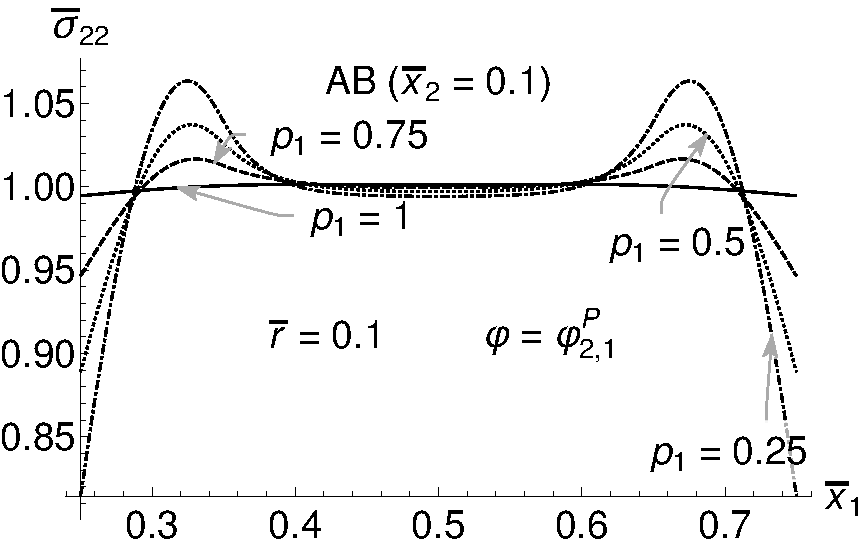
\includegraphics[width=\linewidth]{pics/TStressAB.pdf} \\ а)
        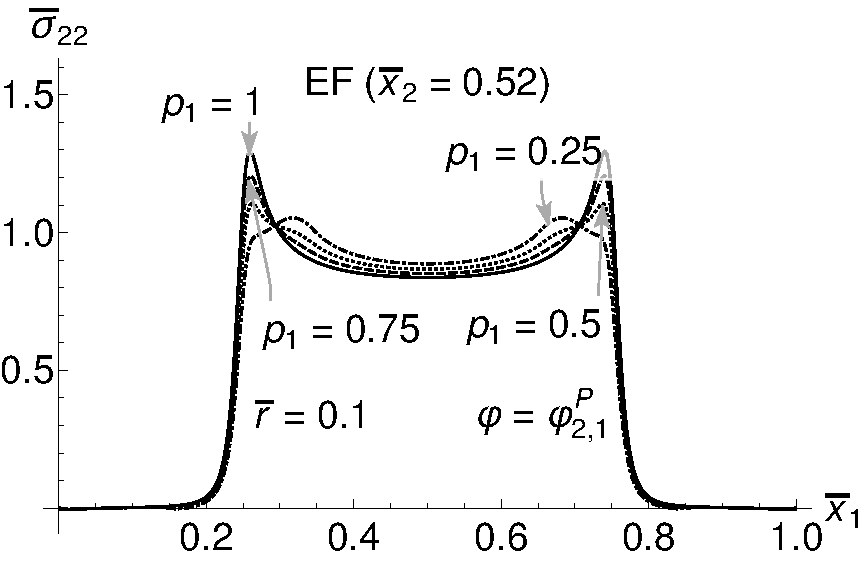
\includegraphics[width=\linewidth]{pics/TStressEF.pdf} \\ в)
    \end{minipage}
    \hfill
    \begin{minipage}[b][][b]{0.49\linewidth}\centering
        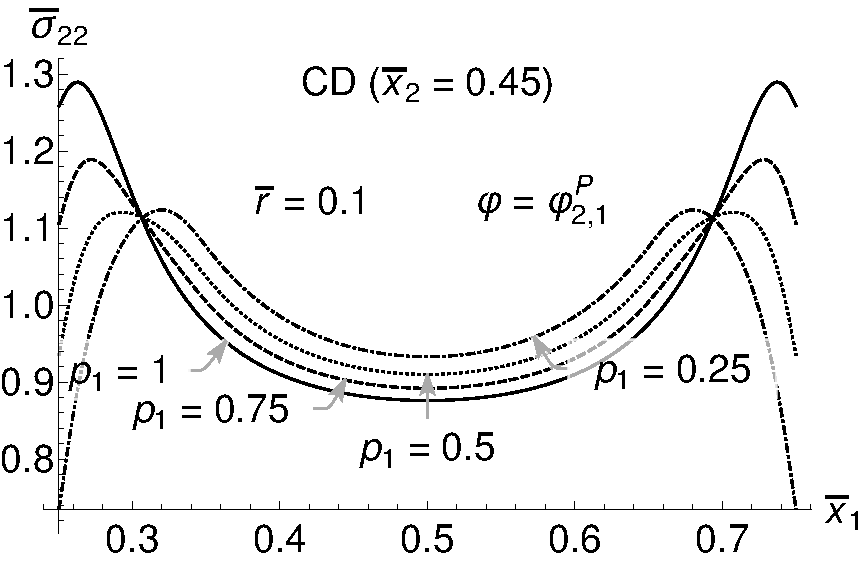
\includegraphics[width=\linewidth]{pics/TStressCD.pdf} \\ б)
        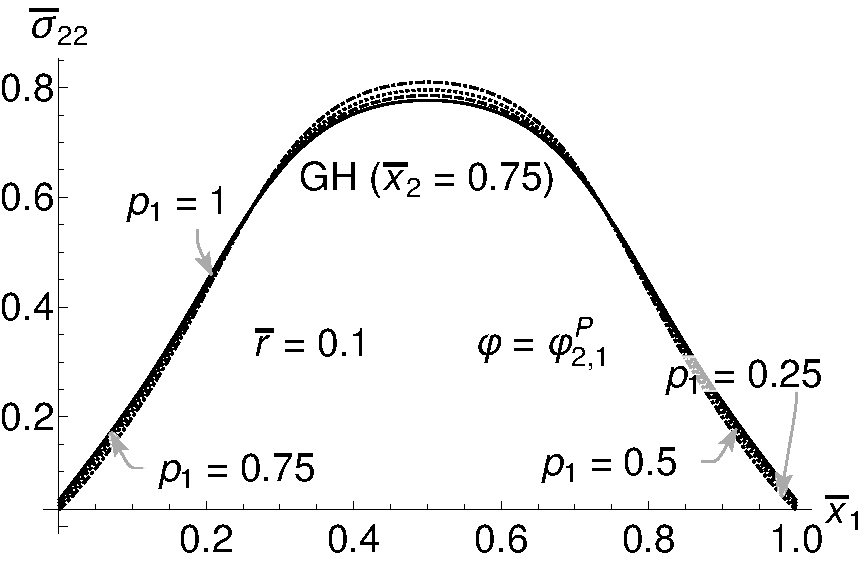
\includegraphics[width=\linewidth]{pics/TStressGH.pdf} \\ г)
    \end{minipage}
    \caption{Распределение напряжений $\overline{\sigma}_{22}$ при различных весовых параметрах $p_1$}
    \label{fig:TSigma}
\end{figure}

\section{Задача Кирша с обобщением на эллиптические вырезы}\label{sec:ResultsAnalysis/KirshProblem}

Продолжим изучение модели на примере решения задачи Кирша с обобщением на эллиптические вырезы. Для этого рассмотрим область $S$, заключённую в квадратную область $\overline{S} = \left\{ \boldsymbol{\overline{x}} \ | \ -1 \leqslant \overline{x}_1, \overline{x}_2 \leqslant 1 \right\}$, с эллиптическим вырезом по центру, где главные оси выреза сонаправлены с осями координат и имеют длины $R_1$ и $R_2$ соответственно. Поставим граничные и геометрические условия
\begin{gather*}
	n_j \overline{\sigma}_{j1} |_{\overline{x}_1 = -1} = -1,
	\quad
	n_j \overline{\sigma}_{j1} |_{\overline{x}_1 = 1} = 1,
	\quad
	\overline{u}_1 |_{\overline{x}_1 = 0} = 0,
	\quad
	\overline{u}_2 |_{\overline{x}_2 = 0} = 0.
\end{gather*}
Схематичное представление области и приложенных нагружений представлены на Рис.~\ref{fig:KirshProblem}, где также введена дополнительная угловая координата $\theta$, необходимая для анализа распределения интересуемых величин на кромке AB. Решение будем искать на структурированной сетке $S_h$, построенной при помощи программного комплекса Abaqus, пример которой при $R_1 = 0.2$ и $R_2 = 0.4$ с характерным размером элементов $h = 0.05$ представлен на Рис.~\ref{fig:KirshMesh}. Расчёты представленные далее были проведены на более подробных сетках с характерным размером элементов $h = 0.005$ при различных параметра $R_1$ и $R_2$ не превышающих 0.1.

\begin{figure}[ht]
    \centerfloat{
        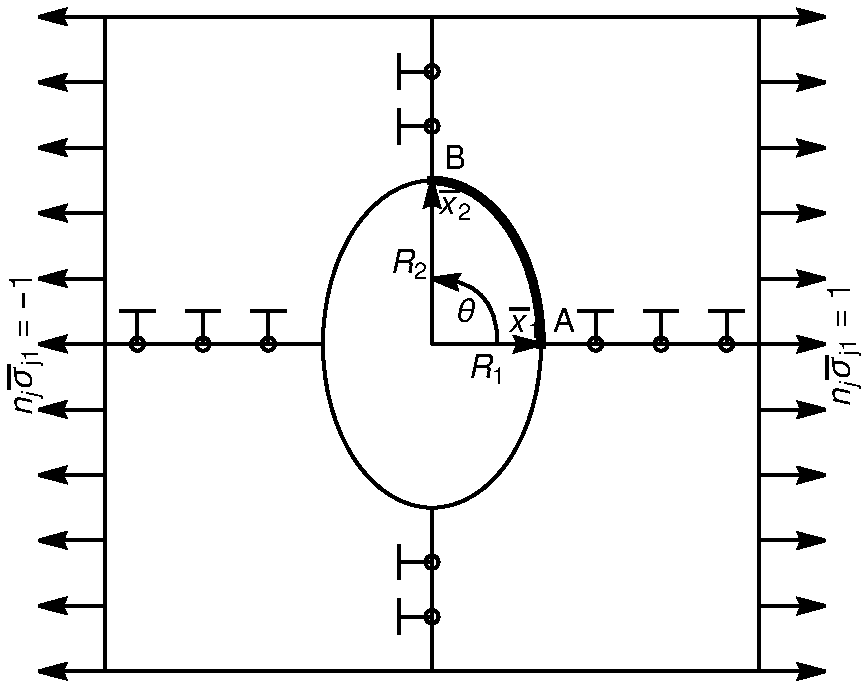
\includegraphics[width=0.7\textwidth]{pics/EllipseStress.pdf}
    }
    \caption{Постановка задачи Кирша}
    \label{fig:KirshProblem}
\end{figure}

\begin{figure}[ht]
    \centerfloat{
        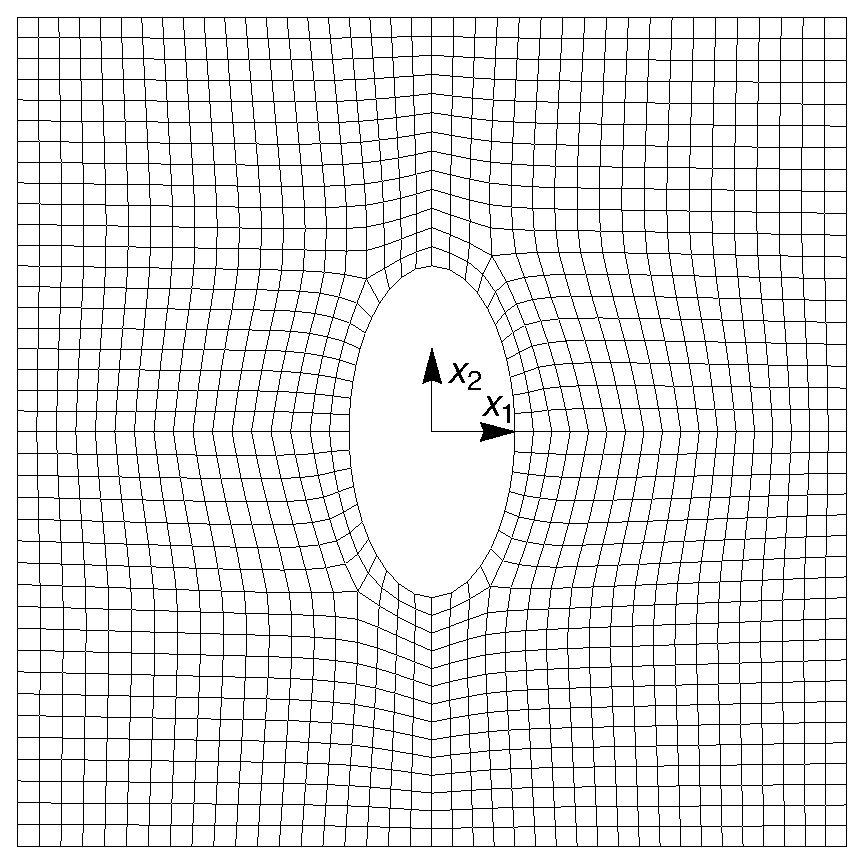
\includegraphics[width=0.7\textwidth]{pics/KirshMesh.pdf}
    }
    \caption{Пример конечно-элементной сетки для обобщённой задачи Кирша}
    \label{fig:KirshMesh}
\end{figure}

Наибольший интерес исследования представляет распределение деформации и напряжений на кромке эллиптического выреза, но так как задача обладает симметрией, сократим рассматриваемую область до дуги AB. Для удобства исследования введём угловой параметр $\theta$, относительно которого параметризуем координаты дуги следующим образом
\begin{gather*}
	\begin{cases}
		x_1 (\theta) = R_1 \cos \theta, \\
		x_2 (\theta) = R_2 \sin \theta,
	\end{cases}
\end{gather*}
где угол $\theta$ принимает значения от 0 до $\pi / 2$. Затем вычислим длину дуги $l$ с зависимостью от угла $\theta$
\begin{gather*}
	l (\theta) = \int\limits_0^{\theta} \sqrt{
		\left( \dfrac{\partial x_1}{\partial \varphi} \right)^2 +
		\left( \dfrac{\partial x_2}{\partial \varphi} \right)^2
	} d \varphi
\end{gather*}
и наконец обезразмерим этот параметр
\begin{gather}
	\label{eq:NaturalParameter}
	\overline{l} (\theta) = \dfrac{l (\theta)}{l \left( \dfrac{\pi}{2} \right)}.
\end{gather}
Дальнейшие результаты на кромке AB будем рассматривать в координатах безразмерного параметра длины $\overline{l}$. В расчётах будем варьировать отношение длин полуосей выреза таким образом, чтобы максимальная длина была равна 0.1, т.е. $\max(R_1, R_2) = 0.1$. Также для дальнейшего анализа введём величину отношения длин полуосей $\rho = R_2 / R_1$.

Для данной постановки задачи известно, что максимальные значения компоненты тензора напряжений $\overline{\sigma}_{11}^{\max}$ находятся в верхней и нижней точках эллипса и образуют линейную зависимость относительно отношения длин полуосей и прикладываемого нагружения \cite{Birger, Bezuh}
\begin{gather*}
	\overline{\sigma}_{11}^{\max} = \left( 1 + 2 \rho \right) \sigma_0,
\end{gather*}
где $\sigma_0$ --- величина прикладываемой нагрузки. Однако в нелокальном случае максимальный уровень напряжения снижается и начинает зависеть ещё и от весового параметра $p_1$. Рассмотрим результаты представленные в \mbox{Таб. \ref{tab:MaxStress}}, где выписаны значения $\overline{\sigma}_{11}^{\max}$ при различных соотношениях длин полуосей эллипса $R_1$ и $R_2$ и весового параметра $p_1$. Заметим, что данные в локальном случае ($p_1 = 1$) хорошо согласуются с представленной выше зависимостью, а в нелокальном необходимо добавить дополнительный множитель $\kappa$, зависящий от весового параметра $p_1$,
\begin{gather*}
	\overline{\sigma}_{11}^{\max} = \kappa \left( 1 + 2 \rho \right) \sigma_0.
\end{gather*}
Такая зависимость не имеет строгого теоретического доказательства и получена эвристически, однако, она может быть полезна для оценки максимальных значений напряжений в практических расчётах. Для оценки параметра $\kappa$ при фиксированном значеним $p_1$ необходимо провести $n$ расчётов при различных соотношениях длин полуосей и выполнить осреднение согласно следующей формуле
\begin{gather}
	\label{eq:Averaging}
	\kappa (p_1) = \dfrac{1}{n} \sum\limits_{i = 0}^{n} \dfrac{\overline{\sigma}_{11}^{\max} (\rho_i, p_1)}{\overline{\sigma}_{11}^{\max} (\rho_i, 1)},
\end{gather}
где $\rho_i$ --- отношение длин полуосей в $i$-ом расчёте. По результатам, представленным в Таб. \ref{tab:MaxStress}, значения $\kappa$ линейно зависят от весового параметра~$p_1$.

\begin{table}[htbp]
    \centering
    \begin{threeparttable}% выравнивание подписи по границам таблицы
        \caption{Максимальный уровень напряжения $\overline{\sigma}_{11}$ при вариации отношения длин полуосей $\rho$ и весового параметра $p_1$, где $\overline{r} = 0.05$}\label{tab:MaxStress}%
        \begin{tabular}{|c|c|c|c|c|}
	        \hline
			Отношение длин    & \multicolumn{4}{c|}{Весовые параметры} \\
			\cline{2-5}
			полуосей $\rho$   & $p_1 = 1$ & $p_1 = 0.75$ & $p_1 = 0.5$ & $p_1 = 0.25$ \\
			\hline
			$0.5$             & 2.012     & 1.783        & 1.537       & 1.510 \\
			\hline
			$0.75$            & 2.578     & 2.235        & 1.919       & 1.727 \\
			\hline
			$1$               & 3.053     & 2.696        & 2.308       & 1.937 \\
			\hline
			$1.25$            & 3.532     & 3.123        & 2.670       & 2.139 \\
			\hline
			$1.5$             & 4.012     & 3.551        & 3.031       & 2.404 \\
			\hline
			$\kappa$          & 1         & 0.881        & 0.755       & 0.652 \\
			\hline
        \end{tabular}
    \end{threeparttable}
\end{table}

Согласно результатам из Таб. \ref{tab:MaxStress}, при $p_1 = 0.75$ и $p_1 = 0.5$ осреднение (\ref{eq:Averaging}) не нужно, так как результаты отношений напряжений в локальном и нелокальном случаях близки при любых значениях $\rho$, представленных в таблице, но при $p_1 = 0.25$ такая зависимость нарушается, однако, при осреднении зависимость параметра $\kappa$ от весового параметра $p_1$ становится близкой к линейной. Разумеется все эти рассуждения требуют более детального теоретического рассмотрения, так как имеющихся эмпирических данных недостаточно для утверждения явных зависимостей.

Вместе с напряжением $\overline{\sigma}_{11}$, при увеличении значения $\rho$, увеличивается и максимальный уровень деформации $\varepsilon_{11}$. Причём если обратить внимание на Рис.~\ref{fig:EpsABLocAndNonloc} то можем заметить, что помимо повышения максимального уровня деформации она также становится более сконцентрированной в верхней и соответственно нижней точках выреза. В нелокальном случае можем наблюдать похожий эффект, однако, здесь также появляется область с отрицательными значениями деформации, которая находится рядом с концентратором. Такой же эффект можно наблюдать при решении нелокальных задач на других областях с концентраторами \cite{ZAMM} и \mbox{экспериментах \cite{Andreev}.}

\begin{figure}[ht]
    \begin{minipage}[b][][b]{0.49\linewidth}\centering
        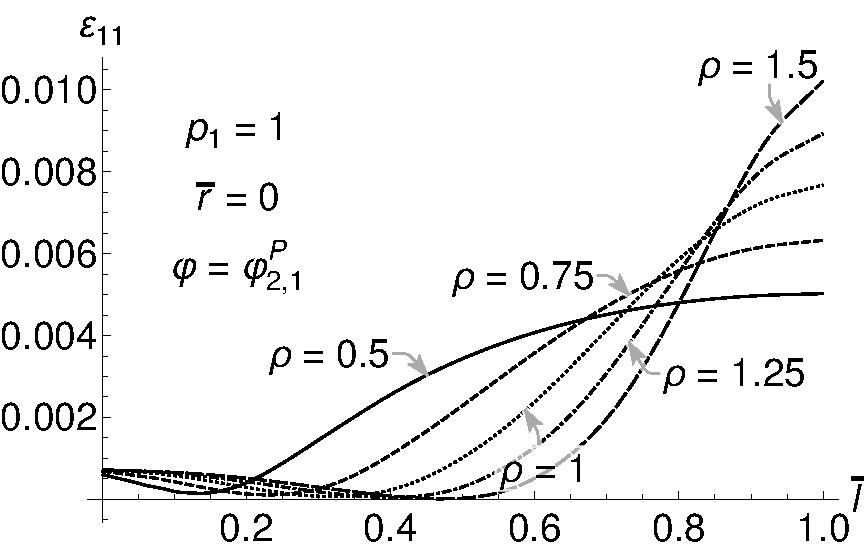
\includegraphics[width=\linewidth]{pics/KirshABEps11Local.pdf} \\ а)
    \end{minipage}
    \hfill
    \begin{minipage}[b][][b]{0.49\linewidth}\centering
        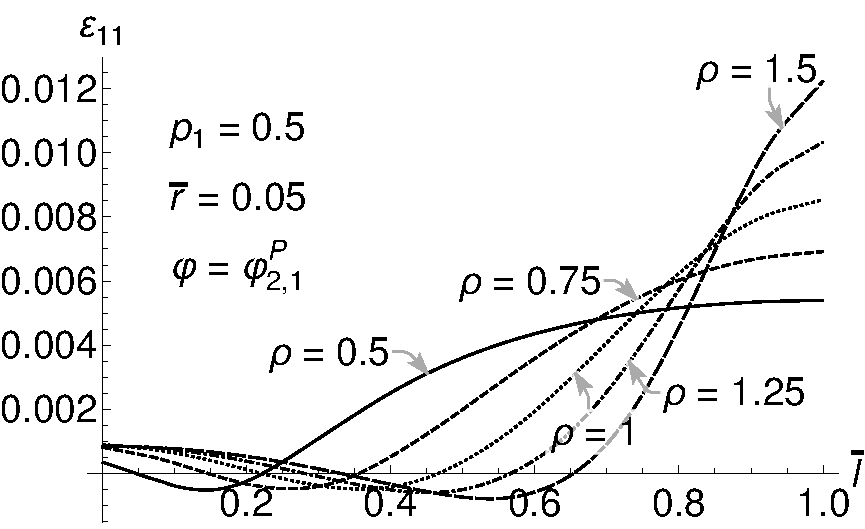
\includegraphics[width=\linewidth]{pics/KirshABEps11r005p05.pdf} \\ б)
    \end{minipage}
    \caption{Распределение компоненты деформации $\varepsilon_{11}$ на кромке AB в (а) локальном и (б) нелокальном случаях при различных соотношениях длин полуосей выреза}
    \label{fig:EpsABLocAndNonloc}
\end{figure}

При уменьшении параметра $p_1$, в отличие от напряжения $\overline{\sigma}_{11}$, деформация $\varepsilon_{11}$ увеличивается в зоне концентрации. Также увеличивается и смежная с ней зона с отрицательными значениями деформации, а сами значения в ней увеличиваются по модулю. Увеличение радиуса нелокальности $\overline{r}$ оказывает похожий  но менее выраженный эффект. Результаты представлены на Рис.~\ref{fig:EpsABVarP1AndR}. В дополнение отметим лишь, что вариация $\overline{r}$ практически не оказывает влияния на величину максимального значения напряжения $\overline{\sigma}_{11}$.

\begin{figure}[ht]
    \begin{minipage}[b][][b]{0.49\linewidth}\centering
        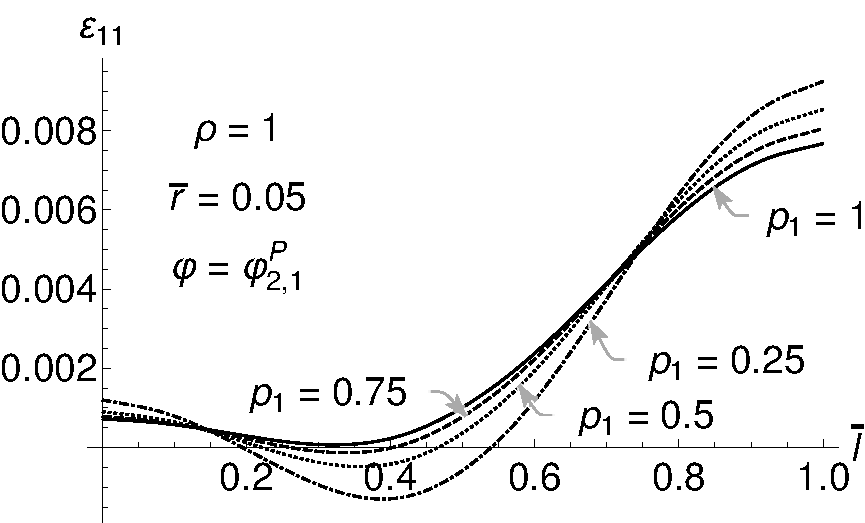
\includegraphics[width=\linewidth]{pics/KirshABEps11VariationP1.pdf} \\ а)
    \end{minipage}
    \hfill
    \begin{minipage}[b][][b]{0.49\linewidth}\centering
        \includegraphics[width=\linewidth]{pics/KirshABEps11VariationR.pdf} \\ б)
    \end{minipage}
    \caption{Распределение компоненты деформации $\varepsilon_{11}$ на кромке AB при вариации (а) весовопого параметра $p_1$ и (б) радиуса нелокальности $\overline{r}$}
    \label{fig:EpsABVarP1AndR}
\end{figure}

\section{Тепловые деформации в областях с эллиптическими вырезами}\label{sec:ResultsAnalysis/ThermalKirshProblem}

Рассмотрим задачу на той же области, что и задачу Кирша, но сменим тип нагружений с механических на тепловые, то есть поставим следующие граничные и геометрические условия
\begin{gather*}
	\boldsymbol{n} \cdot \overline{\boldsymbol{q}}|_{\overline{x}_1 = -1} = 1,
	\quad
	\boldsymbol{n} \cdot \overline{\boldsymbol{q}}|_{\overline{x}_1 = 1} = -1,
	\quad
	\overline{u}_2 |_{\overline{x}_1 = 0} = 0.
\end{gather*}
Графическое изображение постановки задачи представлено на Рис. \ref{fig:ThermalKirshProblem}. Также, для достижения единственности решения, добавим интегральные условия на искомую температуру и первую компоненту вектора перемещения
\begin{gather*}
	\iint\limits_S \overline{T} dS = 0,
	\quad
	\iint\limits_S \overline{u}_1 dS = 0.
\end{gather*}
Такая постановка удобна тем, что позволяет качественно изучить поведение температурных напряжений без появления дополнительных напряжений со стороны возможных концентраторов, обусловленных граничными или геометрическими условиями.

\begin{figure}[ht]
    \centerfloat{
        \includegraphics[width=0.7\textwidth]{pics/EllipseThermal.pdf}
    }
    \caption{Постановка задачи с тепловыми нагружениями}
    \label{fig:ThermalKirshProblem}
\end{figure}

Перед изучением полей напряжений обратим внимание, что аналогично компоненте тензора напряжения $\overline{\sigma}_{11}$ максимальные значения компоненты плотности теплового потока $\overline{q}_1^{\max}$ находятся на верхней и нижней точках эллиптического выреза и они подчинены следующей закономерности
\begin{gather*}
	\overline{q}_1^{\max} = (1 + \rho) q_o,
\end{gather*}
где $q_0$ --- величина подаваемого теплового потока. В нелокальном случае аналогично напряжениям величина $\overline{q}_1^{\max}$ снижается при увеличении вклада нелокального влияния, однако, по результатам представленным в Таб. \ref{tab:MaxFlux} не удаётся также легко определить получившуюся зависимость от $p_1$, так как при весах $p_1 = 0.5$ и $p_1 = 0.25$ и значении $\rho \leqslant 1$ величины $\overline{q}_1^{\max}$ достаточно близки и линейная зависимость от $p_1$ наблюдается только при $\rho = 1.5$.

\begin{table}[htbp]
    \centering
    \begin{threeparttable}% выравнивание подписи по границам таблицы
        \caption{Максимальное значение компоненты теплового потока $\overline{q}_{1}$ при вариации отношения длин полуосей $\rho$ и весового параметра $p_1$, где $\overline{r} = 0.05$}\label{tab:MaxFlux}
        \begin{tabular}{|c|c|c|c|c|}
			\hline
			Отношение длин    & \multicolumn{4}{c|}{Весовые параметры} \\
			\cline{2-5}
			полуосей $\rho$   & $p_1 = 1$ & $p_1 = 0.75$ & $p_1 = 0.5$ & $p_1 = 0.25$ \\
			\hline
			$0.5$             & 1.501     & 1.333        & 1.316       & 1.326 \\
			\hline
			$0.75$            & 1.753     & 1.556        & 1.457       & 1.462  \\
			\hline
			$1$               & 2.001     & 1.781        & 1.597       & 1.591 \\
			\hline
			$1.25$            & 2.252     & 2.002        & 1.734       & 1.644 \\
			\hline
			$1.5$             & 2.494     & 2.222        & 1.927       & 1.681 \\
			\hline
        \end{tabular}
    \end{threeparttable}
\end{table}

Рассмотрим теперь температурные напряжения. Благодаря интегральным условиям, решения получились симметричными и все напряжения сконцентрированы вокруг выреза. Относительно верхней и нижней половин области функции решений чётные, а относительно левой и правой половин нечётные. Зная эти особенности, ограничимся изучением распределения полей напряжения лишь на кромке AB. Для удобства изучения также воспользуемся обезразмеренным параметром длины $\overline{l}$ (\ref{eq:NaturalParameter}).

При вариации параметра $\rho$ кривые $\overline{\sigma}_{11}$ и $\overline{\sigma}_{22}$ существенно изменяют свои формы. На Рис. \ref{fig:ThermalKirshLocal} представлены распределения этих кривых при различных параметрах $\rho$ в классическом случае ($p_1 = 1$). У кривой $\overline{\sigma}_{11}$ вместе с увеличением $\rho$ пиковое значение смещается право вдоль оси O$\overline{l}$. Помимо этого оно также растёт в абсолютных значениях. Максимальная величина $\overline{\sigma}_{22}$ также меняется, но основная закономерность заключается в увеличении площади под кривой при росте $\rho$. Важно отметить, что для обеих кривых в точке $\overline{l} = 1$ их величины равны 0, так как в ней происходит смена знака.

\begin{figure}[ht]
    \begin{minipage}[b][][b]{0.49\linewidth}\centering
        \includegraphics[width=\linewidth]{pics/ThermalKirshSigma11Local.pdf} \\ а)
    \end{minipage}
    \hfill
    \begin{minipage}[b][][b]{0.49\linewidth}\centering
        \includegraphics[width=\linewidth]{pics/ThermalKirshSigma22Local.pdf} \\ б)
    \end{minipage}
    \caption{Распределение напряжения (a) $\overline{\sigma}_{11}$ и (б) $\overline{\sigma}_{22}$ на кромке AB при вариации соотношения длин полуосей}
    \label{fig:ThermalKirshLocal}
\end{figure}

Другими словами, сужение эллиптического выреза вдоль оси O$\overline{x}_1$ приводит к смещению пиковых значений компоненты напряжений $\overline{\sigma}_{11}$ к верхней и нижней точкам выреза, а также увеличению их абсолютных значений. Пиковое значение компоненты напряжений $\overline{\sigma}_{22}$ напротив уменьшается, но при этом занимаемые площади с ненулевыми напряжениями увеличиваются. Таким образом, эллиптические вырезы большая ось которых располагается вдоль линии тока теплового потока дают меньшие напряжения, чем тем, у которых большая ось располагается поперёк.

Учёт нелокальных свойств среды приводит к снижению напряжений $\overline{\sigma}_{11}$ и $\overline{\sigma}_{22}$. Как и во всех расчётах до этого, вариация параметра $\overline{r}$ влияет лишь на форму распределения полей напряжений, а вариация весового параметра $p_1$ на величину отклонения. Распределение полей $\overline{\sigma}_{11}$ и $\overline{\sigma}_{22}$ вдоль кривой AB при вариации $p_1$ представлено на Рис. \ref{fig:ThermalKirshP1Variation}.

\begin{figure}[ht]
    \begin{minipage}[b][][b]{0.49\linewidth}\centering
        \includegraphics[width=\linewidth]{pics/ThermalKirshSigma11VariationP1.pdf} \\ а)
    \end{minipage}
    \hfill
    \begin{minipage}[b][][b]{0.49\linewidth}\centering
        \includegraphics[width=\linewidth]{pics/ThermalKirshSigma22VariationP1.pdf} \\ б)
    \end{minipage}
    \caption{Распределение напряжения (a) $\overline{\sigma}_{11}$ и (б) $\overline{\sigma}_{22}$ на кромке AB при вариации весового параметра $p_1$}
    \label{fig:ThermalKirshP1Variation}
\end{figure}